
%% bare_jrnl.tex
%% V1.4b
%% 2015/08/26
%% by Michael Shell
%% see http://www.michaelshell.org/
%% for current contact information.
%%
%% This is a skeleton file demonstrating the use of IEEEtran.cls
%% (requires IEEEtran.cls version 1.8b or later) with an IEEE
%% journal paper.
%%
%% Support sites:
%% http://www.michaelshell.org/tex/ieeetran/
%% http://www.ctan.org/pkg/ieeetran
%% and
%% http://www.ieee.org/

%%*************************************************************************
%% Legal Notice:
%% This code is offered as-is without any warranty either expressed or
%% implied; without even the implied warranty of MERCHANTABILITY or
%% FITNESS FOR A PARTICULAR PURPOSE!
%% User assumes all risk.
%% In no event shall the IEEE or any contributor to this code be liable for
%% any damages or losses, including, but not limited to, incidental,
%% consequential, or any other damages, resulting from the use or misuse
%% of any information contained here.
%%
%% All comments are the opinions of their respective authors and are not
%% necessarily endorsed by the IEEE.
%%
%% This work is distributed under the LaTeX Project Public License (LPPL)
%% ( http://www.latex-project.org/ ) version 1.3, and may be freely used,
%% distributed and modified. A copy of the LPPL, version 1.3, is included
%% in the base LaTeX documentation of all distributions of LaTeX released
%% 2003/12/01 or later.
%% Retain all contribution notices and credits.
%% ** Modified files should be clearly indicated as such, including  **
%% ** renaming them and changing author support contact information. **
%%*************************************************************************


% *** Authors should verify (and, if needed, correct) their LaTeX system  ***
% *** with the testflow diagnostic prior to trusting their LaTeX platform ***
% *** with production work. The IEEE's font choices and paper sizes can   ***
% *** trigger bugs that do not appear when using other class files.       ***                          ***
% The testflow support page is at:
% http://www.michaelshell.org/tex/testflow/



\documentclass[lettersize,journal]{IEEEtran}
%
% If IEEEtran.cls has not been installed into the LaTeX system files,
% manually specify the path to it like:
% \documentclass[journal]{../sty/IEEEtran}





% Some very useful LaTeX packages include:
% (uncomment the ones you want to load)


% *** MISC UTILITY PACKAGES ***
%
%\usepackage{ifpdf}
% Heiko Oberdiek's ifpdf.sty is very useful if you need conditional
% compilation based on whether the output is pdf or dvi.
% usage:
% \ifpdf
%   % pdf code
% \else
%   % dvi code
% \fi
% The latest version of ifpdf.sty can be obtained from:
% http://www.ctan.org/pkg/ifpdf
% Also, note that IEEEtran.cls V1.7 and later provides a builtin
% \ifCLASSINFOpdf conditional that works the same way.
% When switching from latex to pdflatex and vice-versa, the compiler may
% have to be run twice to clear warning/error messages.






% *** CITATION PACKAGES ***
%
\usepackage{cite}
% cite.sty was written by Donald Arseneau
% V1.6 and later of IEEEtran pre-defines the format of the cite.sty package
% \cite{} output to follow that of the IEEE. Loading the cite package will
% result in citation numbers being automatically sorted and properly
% "compressed/ranged". e.g., [1], [9], [2], [7], [5], [6] without using
% cite.sty will become [1], [2], [5]--[7], [9] using cite.sty. cite.sty's
% \cite will automatically add leading space, if needed. Use cite.sty's
% noadjust option (cite.sty V3.8 and later) if you want to turn this off
% such as if a citation ever needs to be enclosed in parenthesis.
% cite.sty is already installed on most LaTeX systems. Be sure and use
% version 5.0 (2009-03-20) and later if using hyperref.sty.
% The latest version can be obtained at:
% http://www.ctan.org/pkg/cite
% The documentation is contained in the cite.sty file itself.






% *** GRAPHICS RELATED PACKAGES ***
%
\usepackage[pdftex]{graphicx}
\ifCLASSINFOpdf
  % \usepackage[pdftex]{graphicx}
  % declare the path(s) where your graphic files are
  % \graphicspath{{../pdf/}{../jpeg/}}
  % and their extensions so you won't have to specify these with
  % every instance of \includegraphics
  % \DeclareGraphicsExtensions{.pdf,.jpeg,.png}
\else
  % or other class option (dvipsone, dvipdf, if not using dvips). graphicx
  % will default to the driver specified in the system graphics.cfg if no
  % driver is specified.
  % \usepackage[dvips]{graphicx}
  % declare the path(s) where your graphic files are
  % \graphicspath{{../eps/}}
  % and their extensions so you won't have to specify these with
  % every instance of \includegraphics
  % \DeclareGraphicsExtensions{.eps}
\fi
% graphicx was written by David Carlisle and Sebastian Rahtz. It is
% required if you want graphics, photos, etc. graphicx.sty is already
% installed on most LaTeX systems. The latest version and documentation
% can be obtained at:
% http://www.ctan.org/pkg/graphicx
% Another good source of documentation is "Using Imported Graphics in
% LaTeX2e" by Keith Reckdahl which can be found at:
% http://www.ctan.org/pkg/epslatex
%
% latex, and pdflatex in dvi mode, support graphics in encapsulated
% postscript (.eps) format. pdflatex in pdf mode supports graphics
% in .pdf, .jpeg, .png and .mps (metapost) formats. Users should ensure
% that all non-photo figures use a vector format (.eps, .pdf, .mps) and
% not a bitmapped formats (.jpeg, .png). The IEEE frowns on bitmapped formats
% which can result in "jaggedy"/blurry rendering of lines and letters as
% well as large increases in file sizes.
%
% You can find documentation about the pdfTeX application at:
% http://www.tug.org/applications/pdftex





% *** MATH PACKAGES ***
%
\usepackage{amsmath,amssymb}
% A popular package from the American Mathematical Society that provides
% many useful and powerful commands for dealing with mathematics.
%
% Note that the amsmath package sets \interdisplaylinepenalty to 10000
% thus preventing page breaks from occurring within multiline equations. Use:
%\interdisplaylinepenalty=2500
% after loading amsmath to restore such page breaks as IEEEtran.cls normally
% does. amsmath.sty is already installed on most LaTeX systems. The latest
% version and documentation can be obtained at:
% http://www.ctan.org/pkg/amsmath





% *** SPECIALIZED LIST PACKAGES ***
%
%\usepackage{algorithmic}
% algorithmic.sty was written by Peter Williams and Rogerio Brito.
% This package provides an algorithmic environment fo describing algorithms.
% You can use the algorithmic environment in-text or within a figure
% environment to provide for a floating algorithm. Do NOT use the algorithm
% floating environment provided by algorithm.sty (by the same authors) or
% algorithm2e.sty (by Christophe Fiorio) as the IEEE does not use dedicated
% algorithm float types and packages that provide these will not provide
% correct IEEE style captions. The latest version and documentation of
% algorithmic.sty can be obtained at:
% http://www.ctan.org/pkg/algorithms
% Also of interest may be the (relatively newer and more customizable)
% algorithmicx.sty package by Szasz Janos:
% http://www.ctan.org/pkg/algorithmicx




% *** ALIGNMENT PACKAGES ***
%
%\usepackage{array}
% Frank Mittelbach's and David Carlisle's array.sty patches and improves
% the standard LaTeX2e array and tabular environments to provide better
% appearance and additional user controls. As the default LaTeX2e table
% generation code is lacking to the point of almost being broken with
% respect to the quality of the end results, all users are strongly
% advised to use an enhanced (at the very least that provided by array.sty)
% set of table tools. array.sty is already installed on most systems. The
% latest version and documentation can be obtained at:
% http://www.ctan.org/pkg/array


% IEEEtran contains the IEEEeqnarray family of commands that can be used to
% generate multiline equations as well as matrices, tables, etc., of high
% quality.




% *** SUBFIGURE PACKAGES ***
\ifCLASSOPTIONcompsoc
 \usepackage[caption=false,font=normalsize,labelfont=sf,textfont=sf]{subfig}
\else
 \usepackage[caption=false,font=footnotesize]{subfig}
\fi
% subfig.sty, written by Steven Douglas Cochran, is the modern replacement
% for subfigure.sty, the latter of which is no longer maintained and is
% incompatible with some LaTeX packages including fixltx2e. However,
% subfig.sty requires and automatically loads Axel Sommerfeldt's caption.sty
% which will override IEEEtran.cls' handling of captions and this will result
% in non-IEEE style figure/table captions. To prevent this problem, be sure
% and invoke subfig.sty's "caption=false" package option (available since
% subfig.sty version 1.3, 2005/06/28) as this is will preserve IEEEtran.cls
% handling of captions.
% Note that the Computer Society format requires a larger sans serif font
% than the serif footnote size font used in traditional IEEE formatting
% and thus the need to invoke different subfig.sty package options depending
% on whether compsoc mode has been enabled.
%
% The latest version and documentation of subfig.sty can be obtained at:
% http://www.ctan.org/pkg/subfig




% *** FLOAT PACKAGES ***
%
%\usepackage{fixltx2e}
% fixltx2e, the successor to the earlier fix2col.sty, was written by
% Frank Mittelbach and David Carlisle. This package corrects a few problems
% in the LaTeX2e kernel, the most notable of which is that in current
% LaTeX2e releases, the ordering of single and double column floats is not
% guaranteed to be preserved. Thus, an unpatched LaTeX2e can allow a
% single column figure to be placed prior to an earlier double column
% figure.
% Be aware that LaTeX2e kernels dated 2015 and later have fixltx2e.sty's
% corrections already built into the system in which case a warning will
% be issued if an attempt is made to load fixltx2e.sty as it is no longer
% needed.
% The latest version and documentation can be found at:
% http://www.ctan.org/pkg/fixltx2e


%\usepackage{stfloats}
% stfloats.sty was written by Sigitas Tolusis. This package gives LaTeX2e
% the ability to do double column floats at the bottom of the page as well
% as the top. (e.g., "\begin{figure*}[!b]" is not normally possible in
% LaTeX2e). It also provides a command:
%\fnbelowfloat
% to enable the placement of footnotes below bottom floats (the standard
% LaTeX2e kernel puts them above bottom floats). This is an invasive package
% which rewrites many portions of the LaTeX2e float routines. It may not work
% with other packages that modify the LaTeX2e float routines. The latest
% version and documentation can be obtained at:
% http://www.ctan.org/pkg/stfloats
% Do not use the stfloats baselinefloat ability as the IEEE does not allow
% \baselineskip to stretch. Authors submitting work to the IEEE should note
% that the IEEE rarely uses double column equations and that authors should try
% to avoid such use. Do not be tempted to use the cuted.sty or midfloat.sty
% packages (also by Sigitas Tolusis) as the IEEE does not format its papers in
% such ways.
% Do not attempt to use stfloats with fixltx2e as they are incompatible.
% Instead, use Morten Hogholm'a dblfloatfix which combines the features
% of both fixltx2e and stfloats:
%
% \usepackage{dblfloatfix}
% The latest version can be found at:
% http://www.ctan.org/pkg/dblfloatfix




%\ifCLASSOPTIONcaptionsoff
%  \usepackage[nomarkers]{endfloat}
% \let\MYoriglatexcaption\caption
% \renewcommand{\caption}[2][\relax]{\MYoriglatexcaption[#2]{#2}}
%\fi
% endfloat.sty was written by James Darrell McCauley, Jeff Goldberg and
% Axel Sommerfeldt. This package may be useful when used in conjunction with
% IEEEtran.cls'  captionsoff option. Some IEEE journals/societies require that
% submissions have lists of figures/tables at the end of the paper and that
% figures/tables without any captions are placed on a page by themselves at
% the end of the document. If needed, the draftcls IEEEtran class option or
% \CLASSINPUTbaselinestretch interface can be used to increase the line
% spacing as well. Be sure and use the nomarkers option of endfloat to
% prevent endfloat from "marking" where the figures would have been placed
% in the text. The two hack lines of code above are a slight modification of
% that suggested by in the endfloat docs (section 8.4.1) to ensure that
% the full captions always appear in the list of figures/tables - even if
% the user used the short optional argument of \caption[]{}.
% IEEE papers do not typically make use of \caption[]'s optional argument,
% so this should not be an issue. A similar trick can be used to disable
% captions of packages such as subfig.sty that lack options to turn off
% the subcaptions:
% For subfig.sty:
% \let\MYorigsubfloat\subfloat
% \renewcommand{\subfloat}[2][\relax]{\MYorigsubfloat[]{#2}}
% However, the above trick will not work if both optional arguments of
% the \subfloat command are used. Furthermore, there needs to be a
% description of each subfigure *somewhere* and endfloat does not add
% subfigure captions to its list of figures. Thus, the best approach is to
% avoid the use of subfigure captions (many IEEE journals avoid them anyway)
% and instead reference/explain all the subfigures within the main caption.
% The latest version of endfloat.sty and its documentation can obtained at:
% http://www.ctan.org/pkg/endfloat
%
% The IEEEtran \ifCLASSOPTIONcaptionsoff conditional can also be used
% later in the document, say, to conditionally put the References on a
% page by themselves.




% *** PDF, URL AND HYPERLINK PACKAGES ***
%
\usepackage{url}
% url.sty was written by Donald Arseneau. It provides better support for
% handling and breaking URLs. url.sty is already installed on most LaTeX
% systems. The latest version and documentation can be obtained at:
% http://www.ctan.org/pkg/url
% Basically, \url{my_url_here}.




% *** Do not adjust lengths that control margins, column widths, etc. ***
% *** Do not use packages that alter fonts (such as pslatex).         ***
% There should be no need to do such things with IEEEtran.cls V1.6 and later.
% (Unless specifically asked to do so by the journal or conference you plan
% to submit to, of course. )

\usepackage{booktabs}
\usepackage{url,xcolor}

%%%%% NEW MATH DEFINITIONS %%%%%

\usepackage{amsmath,amsfonts,bm}

% Mark sections of captions for referring to divisions of figures
\newcommand{\figleft}{{\em (Left)}}
\newcommand{\figcenter}{{\em (Center)}}
\newcommand{\figright}{{\em (Right)}}
\newcommand{\figtop}{{\em (Top)}}
\newcommand{\figbottom}{{\em (Bottom)}}
\newcommand{\captiona}{{\em (a)}}
\newcommand{\captionb}{{\em (b)}}
\newcommand{\captionc}{{\em (c)}}
\newcommand{\captiond}{{\em (d)}}

% Highlight a newly defined term
\newcommand{\newterm}[1]{{\bf #1}}


% Figure reference, lower-case.
\def\figref#1{figure~\ref{#1}}
% Figure reference, capital. For start of sentence
\def\Figref#1{Figure~\ref{#1}}
\def\twofigref#1#2{figures \ref{#1} and \ref{#2}}
\def\quadfigref#1#2#3#4{figures \ref{#1}, \ref{#2}, \ref{#3} and \ref{#4}}
% Section reference, lower-case.
\def\secref#1{section~\ref{#1}}
% Section reference, capital.
\def\Secref#1{Section~\ref{#1}}
% Reference to two sections.
\def\twosecrefs#1#2{sections \ref{#1} and \ref{#2}}
% Reference to three sections.
\def\secrefs#1#2#3{sections \ref{#1}, \ref{#2} and \ref{#3}}
% Reference to an equation, lower-case.
\def\eqref#1{equation~\ref{#1}}
% Reference to an equation, upper case
\def\Eqref#1{Equation~\ref{#1}}
% A raw reference to an equation---avoid using if possible
\def\plaineqref#1{\ref{#1}}
% Reference to a chapter, lower-case.
\def\chapref#1{chapter~\ref{#1}}
% Reference to an equation, upper case.
\def\Chapref#1{Chapter~\ref{#1}}
% Reference to a range of chapters
\def\rangechapref#1#2{chapters\ref{#1}--\ref{#2}}
% Reference to an algorithm, lower-case.
\def\algref#1{algorithm~\ref{#1}}
% Reference to an algorithm, upper case.
\def\Algref#1{Algorithm~\ref{#1}}
\def\twoalgref#1#2{algorithms \ref{#1} and \ref{#2}}
\def\Twoalgref#1#2{Algorithms \ref{#1} and \ref{#2}}
% Reference to a part, lower case
\def\partref#1{part~\ref{#1}}
% Reference to a part, upper case
\def\Partref#1{Part~\ref{#1}}
\def\twopartref#1#2{parts \ref{#1} and \ref{#2}}

\def\ceil#1{\lceil #1 \rceil}
\def\floor#1{\lfloor #1 \rfloor}
\def\1{\bm{1}}
\newcommand{\train}{\mathcal{D}}
\newcommand{\valid}{\mathcal{D_{\mathrm{valid}}}}
\newcommand{\test}{\mathcal{D_{\mathrm{test}}}}

\def\eps{{\epsilon}}


% Random variables
\def\reta{{\textnormal{$\eta$}}}
\def\ra{{\textnormal{a}}}
\def\rb{{\textnormal{b}}}
\def\rc{{\textnormal{c}}}
\def\rd{{\textnormal{d}}}
\def\re{{\textnormal{e}}}
\def\rf{{\textnormal{f}}}
\def\rg{{\textnormal{g}}}
\def\rh{{\textnormal{h}}}
\def\ri{{\textnormal{i}}}
\def\rj{{\textnormal{j}}}
\def\rk{{\textnormal{k}}}
\def\rl{{\textnormal{l}}}
% rm is already a command, just don't name any random variables m
\def\rn{{\textnormal{n}}}
\def\ro{{\textnormal{o}}}
\def\rp{{\textnormal{p}}}
\def\rq{{\textnormal{q}}}
\def\rr{{\textnormal{r}}}
\def\rs{{\textnormal{s}}}
\def\rt{{\textnormal{t}}}
\def\ru{{\textnormal{u}}}
\def\rv{{\textnormal{v}}}
\def\rw{{\textnormal{w}}}
\def\rx{{\textnormal{x}}}
\def\ry{{\textnormal{y}}}
\def\rz{{\textnormal{z}}}

% Random vectors
\def\rvepsilon{{\mathbf{\epsilon}}}
\def\rvtheta{{\mathbf{\theta}}}
\def\rva{{\mathbf{a}}}
\def\rvb{{\mathbf{b}}}
\def\rvc{{\mathbf{c}}}
\def\rvd{{\mathbf{d}}}
\def\rve{{\mathbf{e}}}
\def\rvf{{\mathbf{f}}}
\def\rvg{{\mathbf{g}}}
\def\rvh{{\mathbf{h}}}
\def\rvu{{\mathbf{i}}}
\def\rvj{{\mathbf{j}}}
\def\rvk{{\mathbf{k}}}
\def\rvl{{\mathbf{l}}}
\def\rvm{{\mathbf{m}}}
\def\rvn{{\mathbf{n}}}
\def\rvo{{\mathbf{o}}}
\def\rvp{{\mathbf{p}}}
\def\rvq{{\mathbf{q}}}
\def\rvr{{\mathbf{r}}}
\def\rvs{{\mathbf{s}}}
\def\rvt{{\mathbf{t}}}
\def\rvu{{\mathbf{u}}}
\def\rvv{{\mathbf{v}}}
\def\rvw{{\mathbf{w}}}
\def\rvx{{\mathbf{x}}}
\def\rvy{{\mathbf{y}}}
\def\rvz{{\mathbf{z}}}

% Elements of random vectors
\def\erva{{\textnormal{a}}}
\def\ervb{{\textnormal{b}}}
\def\ervc{{\textnormal{c}}}
\def\ervd{{\textnormal{d}}}
\def\erve{{\textnormal{e}}}
\def\ervf{{\textnormal{f}}}
\def\ervg{{\textnormal{g}}}
\def\ervh{{\textnormal{h}}}
\def\ervi{{\textnormal{i}}}
\def\ervj{{\textnormal{j}}}
\def\ervk{{\textnormal{k}}}
\def\ervl{{\textnormal{l}}}
\def\ervm{{\textnormal{m}}}
\def\ervn{{\textnormal{n}}}
\def\ervo{{\textnormal{o}}}
\def\ervp{{\textnormal{p}}}
\def\ervq{{\textnormal{q}}}
\def\ervr{{\textnormal{r}}}
\def\ervs{{\textnormal{s}}}
\def\ervt{{\textnormal{t}}}
\def\ervu{{\textnormal{u}}}
\def\ervv{{\textnormal{v}}}
\def\ervw{{\textnormal{w}}}
\def\ervx{{\textnormal{x}}}
\def\ervy{{\textnormal{y}}}
\def\ervz{{\textnormal{z}}}

% Random matrices
\def\rmA{{\mathbf{A}}}
\def\rmB{{\mathbf{B}}}
\def\rmC{{\mathbf{C}}}
\def\rmD{{\mathbf{D}}}
\def\rmE{{\mathbf{E}}}
\def\rmF{{\mathbf{F}}}
\def\rmG{{\mathbf{G}}}
\def\rmH{{\mathbf{H}}}
\def\rmI{{\mathbf{I}}}
\def\rmJ{{\mathbf{J}}}
\def\rmK{{\mathbf{K}}}
\def\rmL{{\mathbf{L}}}
\def\rmM{{\mathbf{M}}}
\def\rmN{{\mathbf{N}}}
\def\rmO{{\mathbf{O}}}
\def\rmP{{\mathbf{P}}}
\def\rmQ{{\mathbf{Q}}}
\def\rmR{{\mathbf{R}}}
\def\rmS{{\mathbf{S}}}
\def\rmT{{\mathbf{T}}}
\def\rmU{{\mathbf{U}}}
\def\rmV{{\mathbf{V}}}
\def\rmW{{\mathbf{W}}}
\def\rmX{{\mathbf{X}}}
\def\rmY{{\mathbf{Y}}}
\def\rmZ{{\mathbf{Z}}}

% Elements of random matrices
\def\ermA{{\textnormal{A}}}
\def\ermB{{\textnormal{B}}}
\def\ermC{{\textnormal{C}}}
\def\ermD{{\textnormal{D}}}
\def\ermE{{\textnormal{E}}}
\def\ermF{{\textnormal{F}}}
\def\ermG{{\textnormal{G}}}
\def\ermH{{\textnormal{H}}}
\def\ermI{{\textnormal{I}}}
\def\ermJ{{\textnormal{J}}}
\def\ermK{{\textnormal{K}}}
\def\ermL{{\textnormal{L}}}
\def\ermM{{\textnormal{M}}}
\def\ermN{{\textnormal{N}}}
\def\ermO{{\textnormal{O}}}
\def\ermP{{\textnormal{P}}}
\def\ermQ{{\textnormal{Q}}}
\def\ermR{{\textnormal{R}}}
\def\ermS{{\textnormal{S}}}
\def\ermT{{\textnormal{T}}}
\def\ermU{{\textnormal{U}}}
\def\ermV{{\textnormal{V}}}
\def\ermW{{\textnormal{W}}}
\def\ermX{{\textnormal{X}}}
\def\ermY{{\textnormal{Y}}}
\def\ermZ{{\textnormal{Z}}}

% Vectors
\def\vzero{{\bm{0}}}
\def\vone{{\bm{1}}}
\def\vmu{{\bm{\mu}}}
\def\vtheta{{\bm{\theta}}}
\def\va{{\bm{a}}}
\def\vb{{\bm{b}}}
\def\vc{{\bm{c}}}
\def\vd{{\bm{d}}}
\def\ve{{\bm{e}}}
\def\vf{{\bm{f}}}
\def\vg{{\bm{g}}}
\def\vh{{\bm{h}}}
\def\vi{{\bm{i}}}
\def\vj{{\bm{j}}}
\def\vk{{\bm{k}}}
\def\vl{{\bm{l}}}
\def\vm{{\bm{m}}}
\def\vn{{\bm{n}}}
\def\vo{{\bm{o}}}
\def\vp{{\bm{p}}}
\def\vq{{\bm{q}}}
\def\vr{{\bm{r}}}
\def\vs{{\bm{s}}}
\def\vt{{\bm{t}}}
\def\vu{{\bm{u}}}
\def\vv{{\bm{v}}}
\def\vw{{\bm{w}}}
\def\vx{{\bm{x}}}
\def\vy{{\bm{y}}}
\def\vz{{\bm{z}}}

% Elements of vectors
\def\evalpha{{\alpha}}
\def\evbeta{{\beta}}
\def\evepsilon{{\epsilon}}
\def\evlambda{{\lambda}}
\def\evomega{{\omega}}
\def\evmu{{\mu}}
\def\evpsi{{\psi}}
\def\evsigma{{\sigma}}
\def\evtheta{{\theta}}
\def\eva{{a}}
\def\evb{{b}}
\def\evc{{c}}
\def\evd{{d}}
\def\eve{{e}}
\def\evf{{f}}
\def\evg{{g}}
\def\evh{{h}}
\def\evi{{i}}
\def\evj{{j}}
\def\evk{{k}}
\def\evl{{l}}
\def\evm{{m}}
\def\evn{{n}}
\def\evo{{o}}
\def\evp{{p}}
\def\evq{{q}}
\def\evr{{r}}
\def\evs{{s}}
\def\evt{{t}}
\def\evu{{u}}
\def\evv{{v}}
\def\evw{{w}}
\def\evx{{x}}
\def\evy{{y}}
\def\evz{{z}}

% Matrix
\def\mA{{\bm{A}}}
\def\mB{{\bm{B}}}
\def\mC{{\bm{C}}}
\def\mD{{\bm{D}}}
\def\mE{{\bm{E}}}
\def\mF{{\bm{F}}}
\def\mG{{\bm{G}}}
\def\mH{{\bm{H}}}
\def\mI{{\bm{I}}}
\def\mJ{{\bm{J}}}
\def\mK{{\bm{K}}}
\def\mL{{\bm{L}}}
\def\mM{{\bm{M}}}
\def\mN{{\bm{N}}}
\def\mO{{\bm{O}}}
\def\mP{{\bm{P}}}
\def\mQ{{\bm{Q}}}
\def\mR{{\bm{R}}}
\def\mS{{\bm{S}}}
\def\mT{{\bm{T}}}
\def\mU{{\bm{U}}}
\def\mV{{\bm{V}}}
\def\mW{{\bm{W}}}
\def\mX{{\bm{X}}}
\def\mY{{\bm{Y}}}
\def\mZ{{\bm{Z}}}
\def\mBeta{{\bm{\beta}}}
\def\mPhi{{\bm{\Phi}}}
\def\mLambda{{\bm{\Lambda}}}
\def\mSigma{{\bm{\Sigma}}}

% Tensor
\DeclareMathAlphabet{\mathsfit}{\encodingdefault}{\sfdefault}{m}{sl}
\SetMathAlphabet{\mathsfit}{bold}{\encodingdefault}{\sfdefault}{bx}{n}
\newcommand{\tens}[1]{\bm{\mathsfit{#1}}}
\def\tA{{\tens{A}}}
\def\tB{{\tens{B}}}
\def\tC{{\tens{C}}}
\def\tD{{\tens{D}}}
\def\tE{{\tens{E}}}
\def\tF{{\tens{F}}}
\def\tG{{\tens{G}}}
\def\tH{{\tens{H}}}
\def\tI{{\tens{I}}}
\def\tJ{{\tens{J}}}
\def\tK{{\tens{K}}}
\def\tL{{\tens{L}}}
\def\tM{{\tens{M}}}
\def\tN{{\tens{N}}}
\def\tO{{\tens{O}}}
\def\tP{{\tens{P}}}
\def\tQ{{\tens{Q}}}
\def\tR{{\tens{R}}}
\def\tS{{\tens{S}}}
\def\tT{{\tens{T}}}
\def\tU{{\tens{U}}}
\def\tV{{\tens{V}}}
\def\tW{{\tens{W}}}
\def\tX{{\tens{X}}}
\def\tY{{\tens{Y}}}
\def\tZ{{\tens{Z}}}


% Graph
\def\gA{{\mathcal{A}}}
\def\gB{{\mathcal{B}}}
\def\gC{{\mathcal{C}}}
\def\gD{{\mathcal{D}}}
\def\gE{{\mathcal{E}}}
\def\gF{{\mathcal{F}}}
\def\gG{{\mathcal{G}}}
\def\gH{{\mathcal{H}}}
\def\gI{{\mathcal{I}}}
\def\gJ{{\mathcal{J}}}
\def\gK{{\mathcal{K}}}
\def\gL{{\mathcal{L}}}
\def\gM{{\mathcal{M}}}
\def\gN{{\mathcal{N}}}
\def\gO{{\mathcal{O}}}
\def\gP{{\mathcal{P}}}
\def\gQ{{\mathcal{Q}}}
\def\gR{{\mathcal{R}}}
\def\gS{{\mathcal{S}}}
\def\gT{{\mathcal{T}}}
\def\gU{{\mathcal{U}}}
\def\gV{{\mathcal{V}}}
\def\gW{{\mathcal{W}}}
\def\gX{{\mathcal{X}}}
\def\gY{{\mathcal{Y}}}
\def\gZ{{\mathcal{Z}}}

% Sets
\def\sA{{\mathbb{A}}}
\def\sB{{\mathbb{B}}}
\def\sC{{\mathbb{C}}}
\def\sD{{\mathbb{D}}}
% Don't use a set called E, because this would be the same as our symbol
% for expectation.
\def\sF{{\mathbb{F}}}
\def\sG{{\mathbb{G}}}
\def\sH{{\mathbb{H}}}
\def\sI{{\mathbb{I}}}
\def\sJ{{\mathbb{J}}}
\def\sK{{\mathbb{K}}}
\def\sL{{\mathbb{L}}}
\def\sM{{\mathbb{M}}}
\def\sN{{\mathbb{N}}}
\def\sO{{\mathbb{O}}}
\def\sP{{\mathbb{P}}}
\def\sQ{{\mathbb{Q}}}
\def\sR{{\mathbb{R}}}
\def\sS{{\mathbb{S}}}
\def\sT{{\mathbb{T}}}
\def\sU{{\mathbb{U}}}
\def\sV{{\mathbb{V}}}
\def\sW{{\mathbb{W}}}
\def\sX{{\mathbb{X}}}
\def\sY{{\mathbb{Y}}}
\def\sZ{{\mathbb{Z}}}

% Entries of a matrix
\def\emLambda{{\Lambda}}
\def\emA{{A}}
\def\emB{{B}}
\def\emC{{C}}
\def\emD{{D}}
\def\emE{{E}}
\def\emF{{F}}
\def\emG{{G}}
\def\emH{{H}}
\def\emI{{I}}
\def\emJ{{J}}
\def\emK{{K}}
\def\emL{{L}}
\def\emM{{M}}
\def\emN{{N}}
\def\emO{{O}}
\def\emP{{P}}
\def\emQ{{Q}}
\def\emR{{R}}
\def\emS{{S}}
\def\emT{{T}}
\def\emU{{U}}
\def\emV{{V}}
\def\emW{{W}}
\def\emX{{X}}
\def\emY{{Y}}
\def\emZ{{Z}}
\def\emSigma{{\Sigma}}

% entries of a tensor
% Same font as tensor, without \bm wrapper
\newcommand{\etens}[1]{\mathsfit{#1}}
\def\etLambda{{\etens{\Lambda}}}
\def\etA{{\etens{A}}}
\def\etB{{\etens{B}}}
\def\etC{{\etens{C}}}
\def\etD{{\etens{D}}}
\def\etE{{\etens{E}}}
\def\etF{{\etens{F}}}
\def\etG{{\etens{G}}}
\def\etH{{\etens{H}}}
\def\etI{{\etens{I}}}
\def\etJ{{\etens{J}}}
\def\etK{{\etens{K}}}
\def\etL{{\etens{L}}}
\def\etM{{\etens{M}}}
\def\etN{{\etens{N}}}
\def\etO{{\etens{O}}}
\def\etP{{\etens{P}}}
\def\etQ{{\etens{Q}}}
\def\etR{{\etens{R}}}
\def\etS{{\etens{S}}}
\def\etT{{\etens{T}}}
\def\etU{{\etens{U}}}
\def\etV{{\etens{V}}}
\def\etW{{\etens{W}}}
\def\etX{{\etens{X}}}
\def\etY{{\etens{Y}}}
\def\etZ{{\etens{Z}}}

% The true underlying data generating distribution
\newcommand{\pdata}{p_{\rm{data}}}
% The empirical distribution defined by the training set
\newcommand{\ptrain}{\hat{p}_{\rm{data}}}
\newcommand{\Ptrain}{\hat{P}_{\rm{data}}}
% The model distribution
\newcommand{\pmodel}{p_{\rm{model}}}
\newcommand{\Pmodel}{P_{\rm{model}}}
\newcommand{\ptildemodel}{\tilde{p}_{\rm{model}}}
% Stochastic autoencoder distributions
\newcommand{\pencode}{p_{\rm{encoder}}}
\newcommand{\pdecode}{p_{\rm{decoder}}}
\newcommand{\precons}{p_{\rm{reconstruct}}}

\newcommand{\laplace}{\mathrm{Laplace}} % Laplace distribution

\newcommand{\E}{\mathbb{E}}
\newcommand{\Ls}{\mathcal{L}}
\newcommand{\R}{\mathbb{R}}
\newcommand{\emp}{\tilde{p}}
\newcommand{\lr}{\alpha}
\newcommand{\reg}{\lambda}
\newcommand{\rect}{\mathrm{rectifier}}
\newcommand{\softmax}{\mathrm{softmax}}
\newcommand{\sigmoid}{\sigma}
\newcommand{\softplus}{\zeta}
\newcommand{\KL}{D_{\mathrm{KL}}}
\newcommand{\Var}{\mathrm{Var}}
\newcommand{\standarderror}{\mathrm{SE}}
\newcommand{\Cov}{\mathrm{Cov}}
% Wolfram Mathworld says $L^2$ is for function spaces and $\ell^2$ is for vectors
% But then they seem to use $L^2$ for vectors throughout the site, and so does
% wikipedia.
\newcommand{\normlzero}{L^0}
\newcommand{\normlone}{L^1}
\newcommand{\normltwo}{L^2}
\newcommand{\normlp}{L^p}
\newcommand{\normmax}{L^\infty}

\newcommand{\parents}{Pa} % See usage in notation.tex. Chosen to match Daphne's book.

\DeclareMathOperator*{\argmax}{arg\,max}
\DeclareMathOperator*{\argmin}{arg\,min}

\DeclareMathOperator{\sign}{sign}
\DeclareMathOperator{\Tr}{Tr}
\let\ab\allowbreak

\newcommand{\fix}{\marginpar{FIX}}
\newcommand{\new}{\marginpar{NEW}}

\newcommand{\ts}{y}
\newcommand{\fullts}{{\bf \ts}}
\newcommand{\tspred}{\hat{\ts}}
\newcommand{\stat}{f}
\newcommand{\statparam}{\theta_{predictor}}
\newcommand{\fullstat}{{\bf \stat}}
\newcommand{\lag}{h}
\newcommand{\window}{w}
\newcommand{\tswindow}{{\bf \ts}}
\newcommand{\meants}{\Bar{\ts}}
\newcommand{\rnnwindow}{{\bf \rnninput}}
\newcommand{\rnninput}{z}
\newcommand{\rnn}{\textsc{rnn}}
\newcommand{\rnnparam}{\theta_{corrector}}
\newcommand{\err}{err}
\newcommand{\errwindow}{{\bf \err}}
\newcommand{\rnnmodel}{\textsc{rnn}}
\newcommand{\ws}{w}
\newcommand{\fullws}{{\bf \ws}}
\newcommand{\wswindow}{{\bf \ws}}
\newcommand{\concatinput}{x}
\newcommand{\fullconcatinput}{{ \bf \concatinput}}
\newcommand{\numberts}{10000}
\newcommand{\threshold}{\eta}
\newcommand{\predictor}{\mathrm{RNN}_p}
\newcommand{\classifier}{\mathrm{RNN}_c}
\newcommand{\remainder}{r}
\newcommand{\hiddenregime}{U}


\begin{document}
%
% paper title
% Titles are generally capitalized except for words such as a, an, and, as,
% at, but, by, for, in, nor, of, on, or, the, to and up, which are usually
% not capitalized unless they are the first or last word of the title.
% Linebreaks \\ can be used within to get better formatting as desired.
% Do not put math or special symbols in the title.
\title{HERMES : Hybrid ERror-corrector Model with inclusion of External Signals for nonstationary fashion time series}
%
%
% author names and IEEE memberships
% note positions of commas and nonbreaking spaces ( ~ ) LaTeX will not break
% a structure at a ~ so this keeps an author's name from being broken across
% two lines.
% use \thanks{} to gain access to the first footnote area
% a separate \thanks must be used for each paragraph as LaTeX2e's \thanks
% was not built to handle multiple paragraphs
%

\author{Etienne David\thanks{Etienne David: Heuritech, France.}, Sylvain Le Corff\thanks{Sylvain Le Corff:  Samovar, T\'el\'ecom SudParis, d\'epartement CITI, TIPIC, Institut Polytechnique de Paris, France.} and~ Jean Bellot\thanks{Jean Bellot: Heuritech, France.}}
%        and~Jane~Doe,~\IEEEmembership{Life~Fellow,~IEEE}% <-this % stops a space
%\thanks{M. Shell was with the Department
%of Electrical and Computer Engineering, Georgia Institute of Technology, Atlanta,
%GA, 30332 USA e-mail: (see http://www.michaelshell.org/contact.html).}% <-this % stops a space
%\thanks{J. Doe and J. Doe are with Anonymous University.}% <-this % stops a space
%\thanks{Manuscript received April 19, 2005; revised August 26, 2015.}}

% note the % following the last \IEEEmembership and also \thanks -
% these prevent an unwanted space from occurring between the last author name
% and the end of the author line. i.e., if you had this:
%
% \author{....lastname \thanks{...} \thanks{...} }
%                     ^------------^------------^----Do not want these spaces!
%
% a space would be appended to the last name and could cause every name on that
% line to be shifted left slightly. This is one of those "LaTeX things". For
% instance, "\textbf{A} \textbf{B}" will typeset as "A B" not "AB". To get
% "AB" then you have to do: "\textbf{A}\textbf{B}"
% \thanks is no different in this regard, so shield the last } of each \thanks
% that ends a line with a % and do not let a space in before the next \thanks.
% Spaces after \IEEEmembership other than the last one are OK (and needed) as
% you are supposed to have spaces between the names. For what it is worth,
% this is a minor point as most people would not even notice if the said evil
% space somehow managed to creep in.



% The paper headers
%\markboth{Journal of \LaTeX\ Class Files,~Vol.~14, No.~8, August~2015}%
%{Shell \MakeLowercase{\textit{et al.}}: Bare Demo of IEEEtran.cls for IEEE Journals}

% The only time the second header will appear is for the odd numbered pages
% after the title page when using the twoside option.
%
% *** Note that you probably will NOT want to include the author's ***
% *** name in the headers of peer review papers.                   ***
% You can use \ifCLASSOPTIONpeerreview for conditional compilation here if
% you desire.




% If you want to put a publisher's ID mark on the page you can do it like
% this:
%\IEEEpubid{0000--0000/00\$00.00~\copyright~2015 IEEE}
% Remember, if you use this you must call \IEEEpubidadjcol in the second
% column for its text to clear the IEEEpubid mark.



% use for special paper notices
%\IEEEspecialpapernotice{(Invited Paper)}




% make the title area
\maketitle

% As a general rule, do not put math, special symbols or citations
% in the abstract or keywords.
\begin{abstract}
Developing models and algorithms to draw causal inference for time series is a long standing statistical problem. It is crucial for many applications, in particular for fashion or retail industries, to make optimal inventory decisions and avoid massive wastes. By tracking thousands of fashion trends on social media with state-of-the-art computer vision approaches, we propose a new model for fashion time series forecasting. Our contribution is  twofold. We first provide the first fashion dataset gathering \numberts\ weekly fashion time series. As influence dynamics are the key of emerging trend detection, we associate with each time series several external weak signals representing behaviors of influencers towards the trend. Secondly, to leverage such a complex and rich dataset, we propose a new hybrid forecasting model. Our approach combines per-time-series parametric models with seasonal components and a global recurrent neural network to include sporadic external signals. This hybrid model provides state-of-the-art results on the fashion dataset, and illustrates the benefit of the contribution of external weak signals.
\end{abstract}

% Note that keywords are not normally used for peerreview papers.
\begin{IEEEkeywords}
Hybrid models, Recurrent neural networks, Time series.
\end{IEEEkeywords}






% For peer review papers, you can put extra information on the cover
% page as needed:
% \ifCLASSOPTIONpeerreview
% \begin{center} \bfseries EDICS Category: 3-BBND \end{center}
% \fi
%
% For peerreview papers, this IEEEtran command inserts a page break and
% creates the second title. It will be ignored for other modes.
\IEEEpeerreviewmaketitle


\section{Introduction}
\label{sec:introduction}

Multivariate time series forecasting is a widespread statistical problem with  many applications, see for instance \cite{sarkka2013bayesian, douc2014nonlinear, zucchini2017hidden} and the numerous references therein.
 %Due to the diversity of applications and use cases, a multitude of models have been proposed. 
 Parametric generative models allow to provide explainable predictions with statistical guarantees based on a precise modeling of the predictive distributions of new data based on a record of past observations. %The parameters of these models are usually estimated using a sequence of observations of the target time series. 
Calibrating these models, for instance using maximum likelihood inference, often requires a fair amount of tuning to design a time series-specific model to provide  accurate forecasts and sharp confidence intervals.  Depending on the use case, statistical properties of the signal and the available data, many families of models have been proposed for time series.  The exponential smoothing model \cite{RePEc:inm:oropre:v:9:y:1961:i:5:p:673-685}, the Trigonometric Box-Cox transform, ARMA errors, Trend, and Seasonal components model (TBATS) \cite{doi:10.1198/jasa.2011.tm09771}, or the ARIMA with the Box-Jenkins approach \cite{box2015time} are for instance very popular parametric linear generative models.  Hidden Markov models (HMM) are also widespread and presuppose that available observations are defined using missing data describing the dynamical system. This hidden state is assumed to be a Markov chain such that at each time step the received observation is a random function of the corresponding latent data.  Although hidden states are modeled as a Markov chain, the observations arising therefrom present a highly complex statistical structure. %Introducing latent hidden states, they assume that the predictive distribution is not unique and constant in time but multiple and lead by the values of the hidden states changing during time. 
 In various applications where signals exhibit non-stationarities such as trends and seasonality, classical HMM are not adapted. However, \cite{touron2017modeling}  recently proposed seasonal HMM, assuming that transition probabilities between the states, as well as the emission distributions, are not constant in time but evolve in a periodic manner. Strong consistency results were established in \cite{touron2019consistency} and Expectation Maximization based numerical experiments were proposed.
Altough these works provide promising results, HMM are computationally expensive to train and are not yet well studied for seasonal  sequences with thousands of components.
 
In many fields, single or few time series have become thousands of sequences with complex statistical structures. In this new context, classical time series specific statistical models show limitations when dealing with numerous heterogeneous data. Recurrent neural networks and recent sequence to sequence deep learning architectures offer very appealing numerical alternatives thanks to their capability of leveraging any kind of heterogeneous multivariate data, see for instance \cite{ hochreiter1997long,vaswani2017attention, 8614252, li2019enhancing, lim2019temporal,salinas2020deepar}.  The DeepAR model proposed in \cite{salinas2020deepar} provides a global model from many time series based on a multi-layer recurrent neural network with LSTM cells. More recently, applications using the Transformer model have been proposed  \cite{li2019enhancing}. A direct concurrent of the DeepAR model can be found with the Temporal Fusion Transformers (TFT) approach \cite{lim2019temporal}.  Unfortunately, all these solutions suffer from two main weaknesses. Firstly, many of them are "black-boxes"  as the final forecast usually does not come with a statistical guarantee  although a few recent works focused on measuring uncertainty in recurrent neural networks, see  \cite{martin2020monte}. Secondly, without a fine prepossessing and well chosen hyper-parameters, these methods may lead to poor results and are often outperformed by traditional statistical models, see \cite{makridakis2018m4}.

In this paper, we consider  new time series forecasting application referred to as {\em fashion trends prediction}. Based on a cutting-edge image recognition technology, we built the first fashion dataset containing \numberts\ sequences representing the apparition of fashion trends on social media per week from 01-01-2015 to 01-01-2019. Our fashion time series has very appealing properties: they have all the same length, same seasonality, no missing value and the absence of sparse time series even for niche trends. The originality of our dataset come from the fact that additional external weak signals can be introduced. With our fashion expertise, we detected several groups of fashion users with a high influence power. Analysing their specific behaviours on social medias, we add to each time series, 4 external weak signals representing the same fashion trends but on a sub-category of users. We call them weak signals because they are often alerts or events that are too sparse, or too incomplete to allow on their own an accurate estimation of their impact on the prediction of the target signal. With this totally new application, we aim at designing a model able to deal with our large fashion dataset, leverage our complex external weak signals and finally provide the most accurate forecasts.
 
Recurrent neural networks are appealing to tackle our forecasting problem due to their capability of leveraging external data.  Recently, hybrid models combining deep neural network (DNN) architectures with widespread statistical models to deal with seasonality and trends have been proposed, see for instance  \cite{zhang2003time,jianwei2019novel,bandara2020lstm}. The approach providing the most striking results was proposed in  \cite{smyl2020hybrid} in the context of the M4 forecasting competition \cite{makridakis2020m4}.  Given a large dataset, a per-time-series multiplicative exponential smoothing model is introduced to estimate simple but fundamental components for each time series and compute a first prediction. Then a global recurrent neural network is trained on the entire dataset to correct errors of the previous exponential smoothing models. 

Following this work, we present in this paper HERMES, a new hybrid recurrent model for time series forecasting with inclusion of external signals. This new architecture is decomposed  into two parts: local predictors and a global corrector.  First, a per-time-series parametric statistical model is trained on all sequences. Then, a global recurrent neural network is trained to evaluate and correct the forecast weaknesses of the first collection of models. By adding external weak signals in the proposed framework, the real potential of the hybrid approach is revealed: a global neural network, able to leverage large amount of heterogeneous data, deal with any kind of external weak signals, learn context and finally correct weaknesses and errors of any parametric models.

The paper is organized as follow. Section~\ref{sec:hybrid} describes the hybrid framework. Then, the new fashion dataset provided with this article is presented in Section~\ref{sec:dataset}. Section~\ref{sec:exp} describes the HERMES results and comparisons with several benchmarks. Finally, a general conclusion and some research perspectives are given in  Section~\ref{sec:conclusion}.

\section{Hybrid model with external signals}
\label{sec:hybrid}
We introduce a new hybrid approach for time series forecasting  composed of two parts: a collection of per-time-series parametric models, the predictors, and a global error-corrector neural network train on all time series, the corrector. Per-time-series parametric models are used to learn local behaviour, to normalize sequences by removing trends and seasonality,  and to compute a first forecast. Then, gathering information of the first predictions and external variables, a recurrent neural networks is trained to correct the predictions provided by the first collection of per-time-series models.

Consider $N\geqslant 1$ time series. For all $1\leqslant n \leqslant N$ and $1\leqslant t \leqslant T$, let $\ts_t^n$ be the value of the $n$-th sequence at time $t$ and  $\fullts^n = \{\ts_t^n\}_{1\leqslant t \leqslant T}$ be all the values of this sequence.   The objective of this paper is to propose a model to  forecast all time series in a given time frame  $\lag \in \mathbb{N}$, i.e. we aim at sampling $\{\ts^n_{T+1:T+\lag}\}_{1\leqslant n \leqslant N}$ based on $\{\ts^n_{1:T}\}_{1\leqslant n \leqslant N}$.


\subsection{Per-time-series predictors}
The time-series-specific predictors compute, for each sequence, a first $\lag$-ahead prediction based on the past. For all $1\leqslant n \leqslant N$, we note $\stat^n(.;\statparam^n)$ the $n$-th parametric model of the $n$-th sequence where $\statparam^n$ are  unknown parameters. Given the sequences $\{\ts^n_{1:T}\}_{1\leqslant n \leqslant N}$ and the estimated  parameters $\{\statparam^n\}_{1\leqslant n \leqslant N}$, the time-series-specific forecasts $\{\tspred^{pred,n}_{T+1:T+\lag|T}\}_{1\leqslant n \leqslant N}$ are, for all $n \in \{1,\ldots,N\}$, for all $i \in \{1,\ldots,\lag\}$,
$$
\tspred^{pred,n}_{T+i|T} = \stat^n(\ts^n_{1:T};\statparam^n)_i\,.
$$

During the M4 competition, the hybrid model of \cite{smyl2020hybrid} was based on a multiplicative exponential smoothing model as the time-series-specific predictor. However, on sporadic time series, this choice leads to poor result and instability. In this paper, a more general framework able to deal with any kind of per-time-series models is provided. In Section~\ref{sec:exp}, two versions of our framework are proposed. The first one use an  exponential smoothing as reference similar to the baseline \cite{smyl2020hybrid} and the second one use a TBATS model \cite{doi:10.1198/jasa.2011.tm09771} which provides better results as this parametric model includes  Fourier representations with time varying coefficients, and ARMA error correction. 

In the specific application of fashion trends prediction, two main forms of standard weaknesses was detected and defined for an univariate parametric forecast as defined above. The first one is a weakness of definition, when the model is not well defined for its forecasting task. For instance, an additive model provide good predictions on time series with additive seasonality but show difficulties with multiplicative one. The second form, harder to detect and correct, is the weakness of information. For non stationary time series, huge changes of behaviours are not always predictable using the past of the sequence. In somes cases, these changes depend on external variables not considered by univariate parametric models. The difficulty is that the exact influence of external variables on the main signal is not mainly know. It is on this point that  the new HERMES framework shows its true potential: introduce a global RNN trained on all the time series and able to consider and leverage external signals. First forecast examples of this new hybrid model are given in Figure~\ref{fig:introexamples}.


\begin{figure*}
\centering
%\begin{subfigure}{1.\textwidth}
 % \centering
  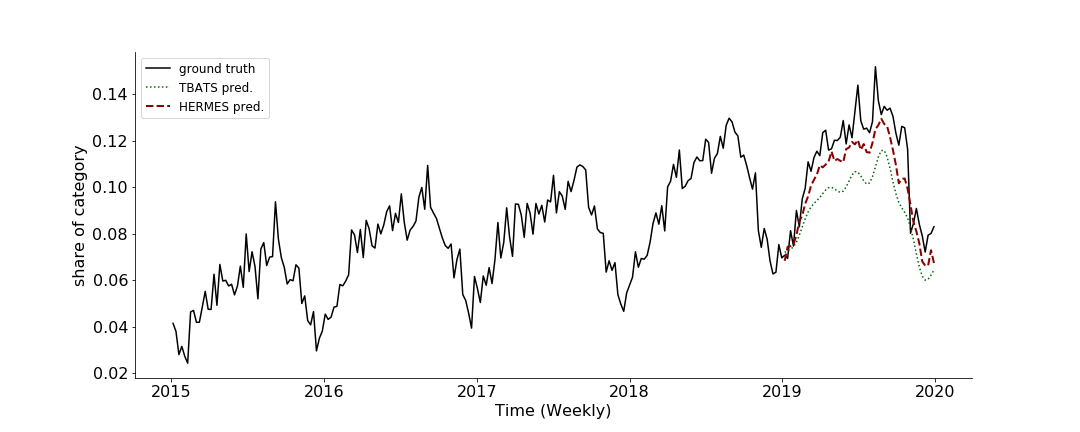
\includegraphics[width=\linewidth]{figure/us_female_shoes}
  %\caption{Time series representing a shoes fashion trend for female in The United States.}
 % \label{fig:introexamples:sub1}
%\end{subfigure}
%\begin{subfigure}{1.\textwidth}
  %\centering
  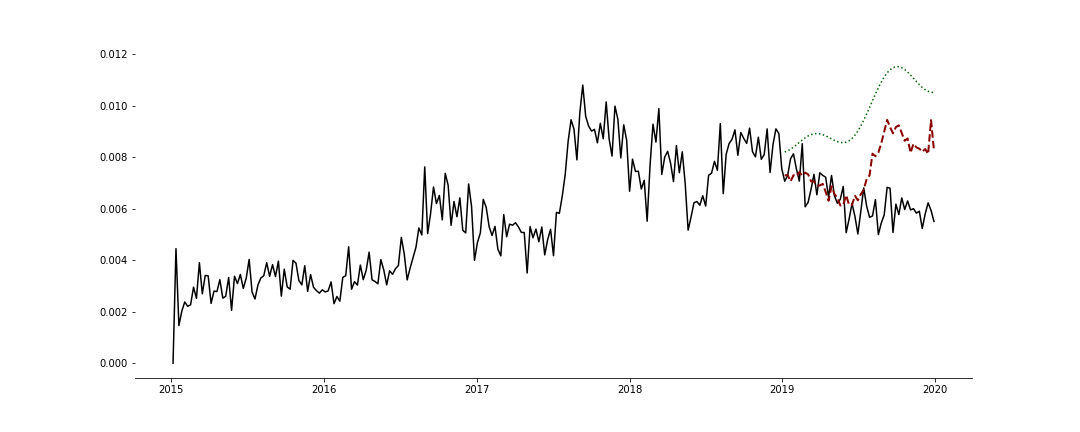
\includegraphics[width=\linewidth]{figure/br_female_texture_verticalstripe}
 % \caption{Time series representing the vertical stipes texture fashion trend for female in Brazil.}
  %\label{fig:introexamples:sub2}
%\end{subfigure}
\caption{Hermes forecast examples. In green the prediction of the TBATS per-time-series predictors. In red the final forecast of our HERMES hybrid model. (Top) Time series representing a shoes fashion trend for female in The United States. (Bottom) Time series representing the vertical stipes texture fashion trend for female in Brazil.}
\label{fig:introexamples}
\end{figure*}

\subsection{Error-corrector recurrent model}

The second part of the model is a global RNN, trained on all the $N$ sequences to correct the weaknesses of the first per-time-series parametric models. This task requires a thorough data pre-processing for two main reasons. First, without a well-design input, the RNN will not be capable of understanding the initial collection of forecasts and predict their future errors. Second, as no assumption about the scale of our time series was made, inputs require a careful normalization before feeding them to the RNN.
Consider the following pre-processing. 


Let $\window \in \mathbb{N}$ be the window size, usually this window is proportional to the forecast horizon $\window \propto \lag$. the RNN input is defined as the following  normalized, deseasonalized and rescaled sequence $\rnnwindow^n_T = \{\rnninput^{n}_{T-\window+i|T}\}_{1\leqslant i \leqslant w}$, where, for all $1\leqslant n \leqslant N$ and $1\leqslant i \leqslant w$, 
$$
\rnninput^{n,T}_{T-w+i|T} = \frac{\ts^n_{T-w+i} -\tspred^{pred,n}_{T+i|T}}{\meants^n_T}\,,\quad \meants^n_T = \frac{1}{w}\sum_{i = 1}^{w}\ts^n_{T-w+i}\,.
$$


Let $\rnn(.;\rnnparam)$ be the recurrent neural network model where $\rnnparam$ are  unknown parameters. Given the RNN input sequences $\{\rnnwindow^n_T\}_{1\leqslant n \leqslant N}$ and the global RNN estimated parameters $\rnnparam$, the error-corrector predictions $\{\tspred^{corr,n}_{T+1:T+\lag|T}\}_{1\leqslant n \leqslant N}$ are, for all $n \in \{1,\ldots,N\}$, for all $i \in \{1,\ldots,\lag\}$,
$$
\tspred^{corr,n}_{T+i|T} = \rnn(\rnnwindow^n_T;\rnnparam)_i \cdot \meants^n_T\ \,.
$$

Our hybrid model forecast is finally given, for all $1\leqslant n \leqslant N$ and all $i \in \{1,\ldots,\lag\}$, by:

\begin{align}
\label{eq:nows:full:model}
\tspred^n_{T+i|T}  &= \tspred^{pred,n}_{T+i|T} +  \tspred^{corr,n}_{T+i|T} \\
&= \stat^n(\ts^n_{1:T};\statparam^n)_i +  \rnn(\rnnwindow^n_T;\rnnparam)_i \cdot \meants^n_T\,.\nonumber
\end{align}


\subsection{Weak signal}

Using well-fitted time-series-specific parametric models, the new hybrid network corrects the first form of weakness and achieves striking accuracy on the provided fashion dataset, see Table~\ref{tab:metricresults}. Then, to correct the second form of weakness, in addition to the $N$ target time series, $K \times N$ external sequences indexed from $0$ to $T$ are considered. For all $1\leqslant n \leqslant N$, $1\leqslant k \leqslant K$ and  $1\leqslant t \leqslant T$, let $\ws^{n,k}_t$ be the value of the $k$-th external sequence at time $t$ linked to the sequence $\fullts^n$. Let  $\fullws^n = \{\{\ws_t^{n,k}\}_{1\leqslant t \leqslant T}\}_{1\leqslant k \leqslant K}$ be all the values of the weak signals linked to the $n$-th sequence. In addition, let $\fullws^n_T = \{\{\ws_{T-w+i}^{n,k}\}_{1\leqslant i \leqslant \window}\}_{1\leqslant k \leqslant K}$ be only the last $\window$ terms of the sequence. Concatenating $ \rnnwindow^n_T$ and $\fullws^n_T$, a new input for the RNN is defined:   
\begin{align*}
\fullconcatinput^n_T &= \{\concatinput^n_{T-w+i|T}\}_{1\leqslant i \leqslant w}\\
&= \{\rnninput^n_{T-w+i|T}, \ws^{n,1}_{T-w+i},...,\ws^{n,K}_{T-w+i}\}_{1\leqslant i \leqslant w}\,.
\end{align*}
Finally, for all $1\leqslant n \leqslant N$ and for all $i \in \{1,\ldots,\lag\}$ the final prediction becomes:
%$$
%\tspred^n_{T+i|T} 
%= \etspred^{ets,n}_{T+i|T} +  \rnnmodel(\fullconcatinput^n_T)_{T+i} \times \meants^n_T
%$$
\begin{align}
\label{eq:withws:full:model}
\tspred^n_{T+i|T}  &= \tspred^{pred,n}_{T+i|T} +  \tspred^{corr,n}_{T+i|T}\\
& = \stat^n(\ts^n_{1:T};\statparam^n)_i +  \rnn(\fullconcatinput^n_T;\rnnparam)_i \cdot \meants^n_T\,.\nonumber
\end{align}
An illustration of the proposed architecture is displayed in Figure~\ref{fig:architecture}.

\begin{figure}
  \centering
    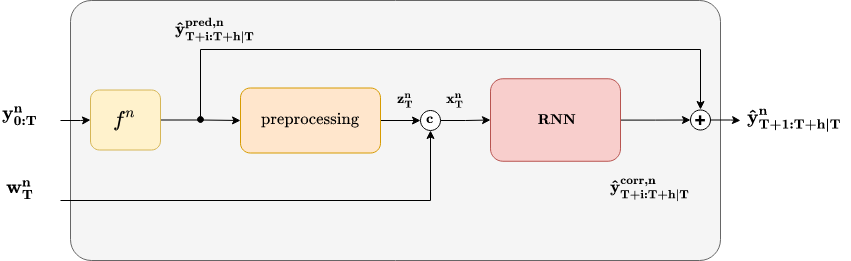
\includegraphics[width=1\linewidth]{figure/HERMES_archi.png}
  \caption{Hybrid model with weak signals architecture.}
\label{fig:architecture}
\end{figure}


\section{Fashion dataset with external weak signals}
\label{sec:dataset}

\subsection{Translate fashion to data}
\label{sec:dataset:a}
A collection of vision neural networks were designed and trained  at detecting clothes details on pictures: type of clothing (pants, shoes, tops, etc.), form, size, color, texture, etc. Then, fashion experts designed fashion trends by aggregating these clothes details: a meaningful combination of items that represent an existing trend in the fashion sphere. To represent finely human behaviors based on social media, a group of thousands of random users, called a panel, was created on several geolocalisations. Analysing every day images shared on social networks by these panels with our computer vision algorithms, we can translate the history of thousands of fashion trends in thousands of time series.  All sequences have 261 time steps, from 2015-01-05 to 2019-12-31 with weekly values and no missing values. Each value represents the number of users posts in a week where vision algorithms detected the fashion trend on picture.  As an illustration, an example of fashion time series is given in Figure~\ref{fig:normalization}.

\subsection{Fashion dataset}
\label{sec:dataset:b}

Due to the increasing use of social media and users change of behaviour, a normalization step is applied to the raw sequences. Each fashion trend is divided by its hierarchical parent category trend. Moreover, in order not to remove the seasonality of all sequences, we deseasonalized the hierarchical parent category trend before the normalization. For instance, as displayed in Figure~\ref{fig:normalization}, the raw Jersey Top trend for female in China is divided by the deseasonalized global Top trend for female in China. The final normalized sequence is expressed in share of category.

We therefore introduce a new dataset for fashion time series forecasting.  It contains a sample of $\numberts$ anonymized and  normalized fashion trends for men and women, on 9 different categories and 5 geozones. An overview of it can be found in Table~\ref{tab:fashiondataset}. this collection of $\numberts$ fashion trends was selected in order to represent finely the issues faced by the fashion industry. For instance, some sequences show complex behaviours with sudden changes. They are called emerging or declining trends depending on the change in direction. A central point of this work is to accurately detect and forecast such trends.

\begin{figure*}
\centering
%\begin{subfigure}{1.\textwidth}
 % \centering
  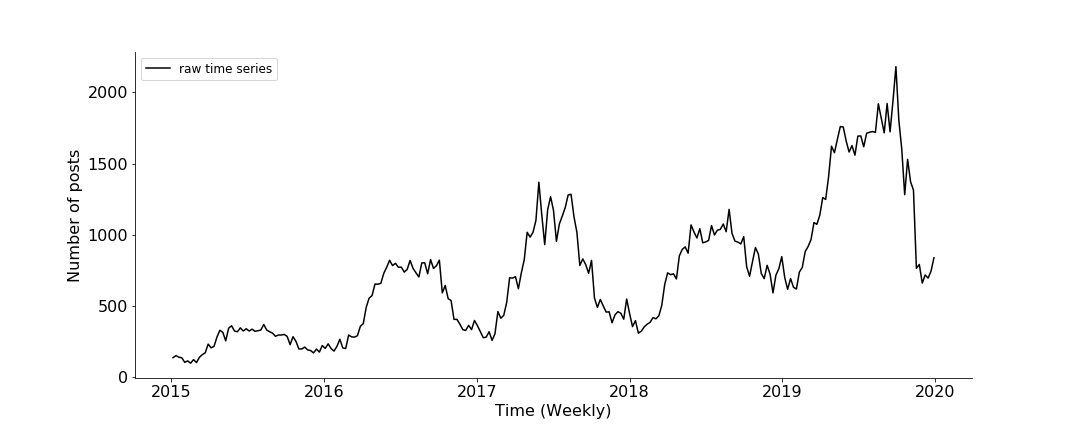
\includegraphics[width=1.\linewidth]{figure/cn_female_top_raw}
%  \caption{Time series representing the raw signal of a top fashion trend for female in China}
 % \label{fig:normalization:sub1}
%\end{subfigure}
%\begin{subfigure}{1.\textwidth}
 % \centering
  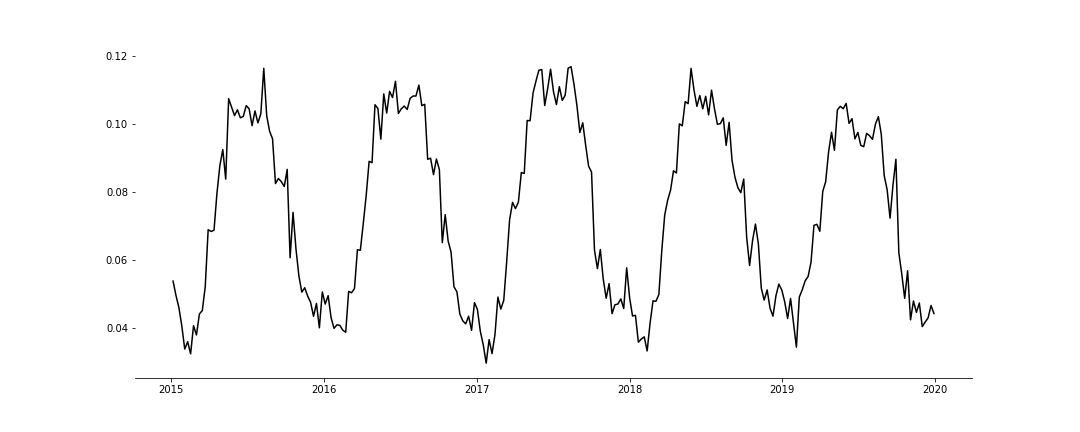
\includegraphics[width=1.\linewidth]{figure/cn_female_top_norm}
  %\caption{Time series representing the normalized signal of a top fashion trend for female in China.}
  %\label{fig:normalization:sub2}
%\end{subfigure}
\caption{Example of difference between the raw sequence and the normalized one. In this example, we normalize by the deseasonalized global top fashion trend for female in China. (Top) Time series representing the raw signal of a top fashion trend for female in China. (Bottom) Time series representing the normalized signal of a top fashion trend for female in China.}
\label{fig:normalization}
\end{figure*}

\begin{table*}
  \caption{Fashion time series overview. For each couple geozone/category, we give the number of female and male trends (Female/Male).}
\label{tab:fashiondataset}
  \centering
  \resizebox{0.85\width}{!}{
  \begin{tabular}{l||lllllllll}
    %hline
    \\
    &  \textbf{Top}  & \textbf{Pants} & \textbf{Short} & \textbf{Skirt} & \textbf{Dress} & \textbf{Coat} & \textbf{Shoes} & \textbf{Color} & \textbf{Texture}  \\
    \hline
    \hline
    \\
\textbf{United States} & 411/208 & 149/112 & 47/22 & 29/- & 20/- & 208/151 & 293/86 & 38/44 & 85/81\\
     \textbf{Europe} & 409/228 &  134/114 & 48/21 & 28/- & 20/- & 211/159 & 303/78 & 41/42 & 87/74\\
     \textbf{Japan} &  403/218 & 136/107 & 49/31 & 28/- &  23/- & 185/149 &  311/78 & 46/42 &  92/65\\
     \textbf{China} &  424/202 & 147/114 & 46/29 & 27/- &  27/- & 178/161 &  310/78 & 41/47 &  88/77\\
     \textbf{Brazil} &  431/222 & 134/117 & 49/27 & 30/- &  28/- & 203/152 & 311/76 & 48/41 & 107/84\\
     \\
     %\hline
     \textbf{Total} & 2078/1078 & 700/564 & 239/130 & 142/- & 118/- & 985/772 & 1528/396 & 214/216 & 459/381\\
    %\hline
  \end{tabular}
  }
\end{table*}

\subsection{Weak signal}

In theoretical fashion dynamics \cite{rogersdiffusion}, different categories of adopters follow a trend in succession, resulting in several adoption waves. In this way, several weak signals for each sequence are added to the proposed large dataset.

Firstly, numerous social media influencers were selectioned by hand by fashion experts. By aggregating them, a specific ``fashion-oriented`` panel is created. With the same methodology than for the main panel descibed in Section~\ref{sec:dataset:a} and Section~\ref{sec:dataset:b}, a normalized time series representing each fashion trend on this specific population is created. We named \textit{fashion-forwards} this first weak signal.  For all trend $\{y_t\}_{1\leqslant t\leqslant T}$, let $\ts_t^{f,n}$ be the value of the $n$-th \textit{fashion-forwards} sequence at time $t$ and  $\fullts^{f,n} = \{\ts_t^{f,n}\}_{1\leqslant t \leqslant T}$ be all the values of this sequence.
As we want to detect shifts between the main signal and the fashion forward signal, the following input is computed for our hybrid model:  for all $n \in \{1,\ldots,N\}$, for all $t \in \{1,\ldots,T\}$,
$$
\ws^{f,n}_{t} = \frac{\ts_t^{f,n}}{\ts_t^{f,n}+\ts_t^{n}}\,.
$$
Values close to 0.5 indicate a similar behaviour between the influencers panel and the general panel. For instance, an impressive emerging fashion shoes trend with its linked \textit{fashion-forwards} weak signal is represented in Figure~\ref{fig:oneemergingtrend}. 


Secondly, depending of the number of followers, the general panel of users is divided in three sub-groups: users with less than 1350 followers, users with a number of followers between 1350 and 7000 and users with more than 7000 followers. Repeating the previous methodology on each sub-panel, three normalized time series for each time series are created.  Again, the motivation here is to detect behaviour gaps between different part of the society that could announce bigger changes in the main signal. Let $\ts_t^{\ell,n}$,$\ts_t^{m,n}$ and $\ts_t^{h,n}$ be the value of the $n$-th \textit{followers-low},\textit{followers-mid} and \textit{followers-high} sequence at time $t$ and  $\fullts^{\ell,n} = \{\ts_t^{f,n}\}_{1\leqslant t \leqslant T}$, $\fullts^{m,n} = \{\ts_t^{f,n}\}_{1\leqslant t \leqslant T}$, $\fullts^{h,n} = \{\ts_t^{f,n}\}_{1\leqslant t \leqslant T}$ be all the values of these sequences. Two inputs for our hybrid model are computed: for all $n \in \{1,\ldots,N\}$, for all $t \in \{1,\ldots,T\}$,
\begin{align*}
\ws^{\ell,n}_{t} = \frac{\ts_t^{\ell,n}}{\ts_t^{\ell,n}+\ts_t^{m,n}+\ts_t^{h,n}}\,,\quad \ws^{h,n}_{t} = \frac{\ts_t^{h,n}}{\ts_t^{\ell,n}+\ts_t^{m,n}+\ts_t^{h,n}}
\end{align*}  
values close to 0.3 indicate a similar behaviour between the three sub-panels and the general panel.

In addition to the fashion dataset, for each time series, the three weak signals $\ws^{f}$,$\ws^{\ell}$ and $\ws^{h}$ are added. They are frequently sparse for micro trends and they often lack interest in common fashion trends. However, in several examples, they are fundamental to detect the future fashion evolutions, as illustrated in Section~\ref{sec:exp}. 


\begin{figure*}
  \centering
    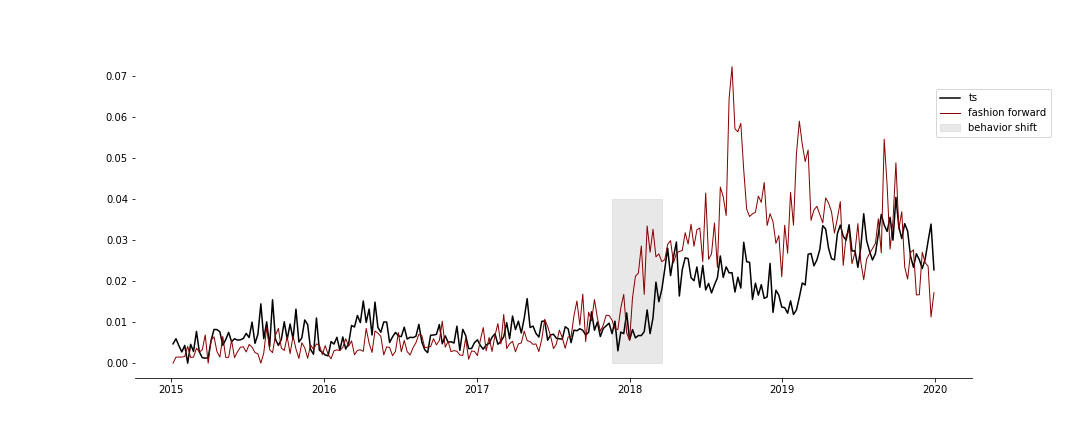
\includegraphics[width=1.\linewidth]{figure/ff_example}
  \caption{A shoes trend of the fashion dataset. In black the main signal and in red its associated \textit{fashion-forward} weak signal. The shift between these two signals at the end of 2017/beginning of 2018 announces the future burst of the trend.}
\label{fig:oneemergingtrend}
\end{figure*}





\section{Experimental results}
\label{sec:exp}

\subsection{Training}

The dataset is temporally split into three blocks, {\em train}, {\em eval} and {\em test} sets. The 3 first years are used as the {\em train} set, the 4th year is kept for the {\em eval} set and the {\em test} set is made of the last year. The hyrid model is trained to compute a one-year ahead prediction, $\lag$ equal to 52, and the window size $\window$ is fixed at 104.
Using the two first year of the {\em train} set, a first per-time-series parametric model for each time series is fitted. With the resulting collection of local models, a forecast of the third year is computed for each sequence. Corrector inputs are finally computed and the RNN is trained at correcting weaknesses of this first collection of third-year forecasts. For the {\em eval} set, per-time-series predictors are fitted a second time using the three first years and a forecasts of the fourth year are computed. The {\em eval} set is used during the training to control the learning of the RNN model and prevent overfitting. The per-time-series predictors are fitted a last time for the {\em test} set using the four first years. The final accuracy measures of all our models are computed on this {\em test} set. As an illustration, an example of our temporal split is shown in Figure~\ref{fig:train_eval_test_set}.

For the first parametric per-time-series models, existing Python or R libraries are used to estimate the different parameters $\statparam^n$.  Depending of the choice of local parametric models, two versions of HERMES are proposed. The first one uses as predictors an additive exponential smoothing model as a reference close to \cite{smyl2020hybrid}. The second one uses the TBATS model of \cite{doi:10.1198/jasa.2011.tm09771} and  achieves striking accuracy results on the fashion dataset. The neural network part architecture is summarized in Figure~\ref{fig:rnn_architecture}. It is composed of 3 LSTM layer of shape 50 and a final Dense layer to provide the correct output dimension. A classical Adam optimizer is used with a learning rate set at 0.001 or 0.005, the batch size is fixed 64 and the loss function is defined as follows:
$$
\ell(\ts^n_{T+1:T+\lag},\tspred^n_{T+1:T+\lag|T}) = \frac{1}{\meants^n_T}\sum_{i=1}^{\lag}|\ts^n_{T+i} - \tspred^n_{T+i|T}|\,.
$$
This choice of $\mathrm{L}_1$  loss function is motivated by its robustness to outliers which accounts for some time series in the fashion industry with very specific behaviors. The loss and previous parameters are all set with a grid search (additional materials can be found in Appendix). the code is developed in Python using the Tensorflow library. It allows the use of a GPU to speed up the trainig process.



\begin{figure*}
  \centering
    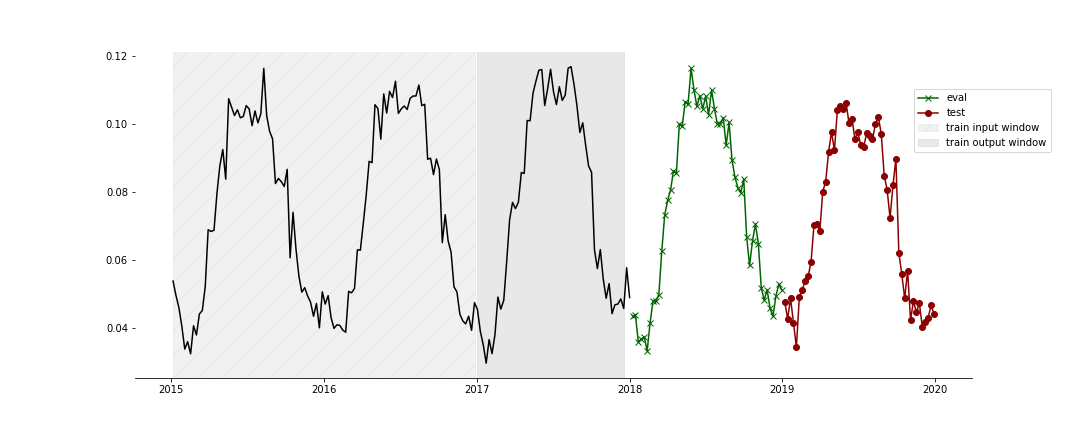
\includegraphics[width=1.\linewidth]{figure/train_eval_test_set}
  \caption{Temporal split for our training process}
\label{fig:train_eval_test_set}
\end{figure*}

\begin{figure}
  \centering
    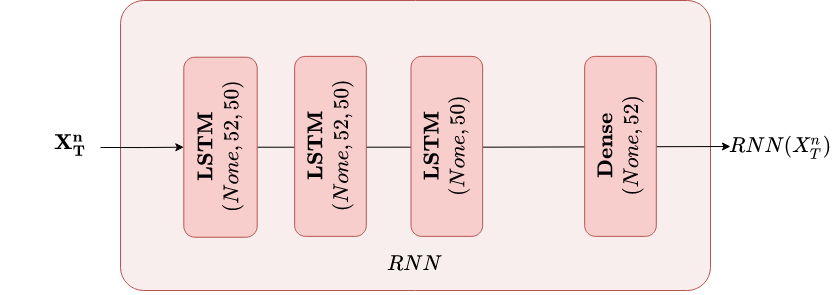
\includegraphics[width=0.8\linewidth]{figure/lstm_archi}
  \caption{$\classifier$ and $\predictor$ architecture.}
\label{fig:rnn_architecture}
\end{figure}

\subsection{Benchmarks, hybrid models and Metrics}

As benchmarks, several widespread statistical methods and deep learning approaches were selected. Using the R package \texttt{forecast} and the Python packages \texttt{statsmodels},  \texttt{tbats}, for each time series, predictions are computed with the following methods: \textit{snaive}, \textit{ets}, \textit{stlm}, \textit{thetam}, \textit{tbats} and \textit{auto.arima}. The forecast of the \textit{snaive} method is only the repetition of the last same past period. The \textit{ets} model is an additive exponential smoothing with a level component and a seasonal component. The \textit{stlm} approach uses a multiplicative decomposition and models the seasonally adjusted time series with an exponential smoothing model. The \textit{Thetam} model decomposes the original signal in $\theta$-lines, predicts each one separately and recomposes them to produce the final forecast and \textit{tbats} is a powerful statistical model using a trigonometrical seasonality modelization. Finally, \textit{auto.arima} is the R implementation of the ARIMA model with an automatic selection of the best parameters. A complete description and references for these models can be found in \cite{hyndman2020package}. As a deep learning approach, a full LSTM (\textit{lstm}) neural network composed of 3 LSTM layers of shape 50 and a final Dense layer of shape 52 is considered.
Two versions of HERMES are proposed. They are called respectively \textit{hermes-ets} and \textit{hermes-tbats} according to the per-time-series model choice. Moreover, two versions with the inclusion of the weak signals (ws) are proposed. They are referred as \textit{hermes-ets-ws} and \textit{hermes-tbats-ws}. In order to provide a fair comparison, a \textit{lstm} with the weak signals named \textit{lstm-ws} is trained.

To compare the different methods, we use the Mean Absolute Scaled Error (MASE). As our time series have complete different scale, from $10^{-5}$ to $10^{-1}$, this metric was chosen to compute a fair error measure, independent of the scale of the sequence. The MASE metric is defined as follows:
\begin{align*}
\mathrm{MASE} &= \frac{T-m}{h}\frac{\sum_{i=1}^h |Y_i - \hat{Y}_i| }{\sum_{i=1}^{T-m} |Y_i - Y_{i-m}|}
\end{align*}
Detecting emerging and declining trends is a crucial issue for the fashion industry. A correct or incorrect prediction could lead to good returns or massive waste due to overstock or unsold clothes. In addition to the MASE accuracy metric, the different methods are also evaluated on a classification task and especially difference between methods using weak signals or not. In a given year, an increasing trend is defined as a trend that does more than 5\% of growth with respect to the previous year. In the same way, a decreasing trend is defined as a trend that declines by 5\% or more. Other trends are classified as flat trends. With this threshold, the proposed fashion dataset is almost balanced on the {\em test} set: There are 3087 increasing trends, 3342 decreasing trends and 3571 flat trends. On the {\em test} set, for each method, the accuracy is defined as follows:
\begin{align*}
\mathrm{ACCURACY} &= \frac{TP}{TP + FP}\,,
\end{align*}
where $TP = TP_{dec} + TP_{flat} + TP_{inc}$ and $FP = FP_{dec} + FP_{flat} + FP_{inc}$ with $TP_i$  the number of time series correctly classified in the class $i$ and $FP_i$ the number of time series miss classified in the class $i$.


\subsection{Result for Heuritech Fashion dataset}

\textbf{10000 Heuritech Fashion time series global accuracy. }For the two metrics and for each model, we compute the average on all our sequences \numberts~  on the final year. Results are displayed in the Table~\ref{tab:metricresults}. For our model using neural networks, 10 models are trained  with different seeds. The average and the standard deviation of their results are computed and displayed. For the statistical models, TBATS largely dominates the alternatives  in terms of MASE. It is one of the main motivations why this model is used on the best HERMES candidate as the predictor model. 

Considering the new HERMES approach, \textit{hermes-tbats} and \textit{hermes-tbats-ws} slighlty outperform the alternatives in terms of MASE and are stable across the different trainings. Regarding \textit{hermes-ets},   although it is very similar to the baseline \cite{smyl2020hybrid}, its accuracy remains low in comparison to the \textit{lstm} benchmarck or HERMES using TBATS. 

Models using our weak signals perform similarly as without-weak-signals models for the MASE. In Figure~\ref{fig:introexamples}. Interestingly, weak signals sinificantly improve the accuracy in detecting emerging and declining trends. Figure~\ref{fig:examples} displays some examples of \textit{hermes-tbats} model and some weaknessess that can be corrected.

\begin{table}
  \caption{Results summary on the 10000ts Fashion dataset. For each metric, the average on all our time series is computed. For approaches using neural network, 10 models are trained with different seeds. The mean and the standard deviation of the 10 results are displayed.}
  \centering
%  \resizebox{0.85\textwidth}{!}{%
  \begin{tabular}{l||lllll|lllll}
   &&\multicolumn{3}{c}{\textbf{MASE}} &&& \multicolumn{3}{c}{\textbf{ACCURACY}}&\\
    &&  \textit{mean}  && \textit{std} &&&  \textit{mean}  && \textit{std}& \\
%    \hline
	 \hline
	 &&&&&&&&&&\\
     \textit{snaive} && 0.881 && - &&& 0.357 && - &\\
     \textit{thetam}  && 0.844 && -&&& 0.482 && - &\\
     \textit{arima} && 0.826 && -&&& 0.464 && - & \\
     \textit{ets} && 0.805 && -&&& 0.449 && - & \\
     \textit{stlm} && 0.770 && -&&& 0.482 && - & \\
     \textit{hermes-ets-ws} && 0.769 && 0.005 &&& 0.501 && 0.007 &\\
     \textit{hermes-ets} && 0.758 && 0.001 &&& 0.490 && 0.006 &\\
     \textit{tbats} && 0.745 && -&&& 0.453 && - & \\
     \textit{lstm-ws} && 0.728 && 0.004 &&& 0.500 && 0.008 &\\
     \textit{lstm} && 0.724 && 0.003 &&& 0.498 && 0.007 &\\
     \textit{hermes-tbats} && 0.715 && 0.002 &&& 0.488 && 0.008 &\\
     \textbf{\textit{hermes-tbats-ws}} && \textbf{0.712} && 0.004 &&& \textbf{0.510} && 0.005 &\\
    %\hline
  \end{tabular}
%  }
\label{tab:metricresults}
\end{table}

\begin{figure*}
\centering
%\begin{subfigure}{1.\textwidth}
 % \centering
  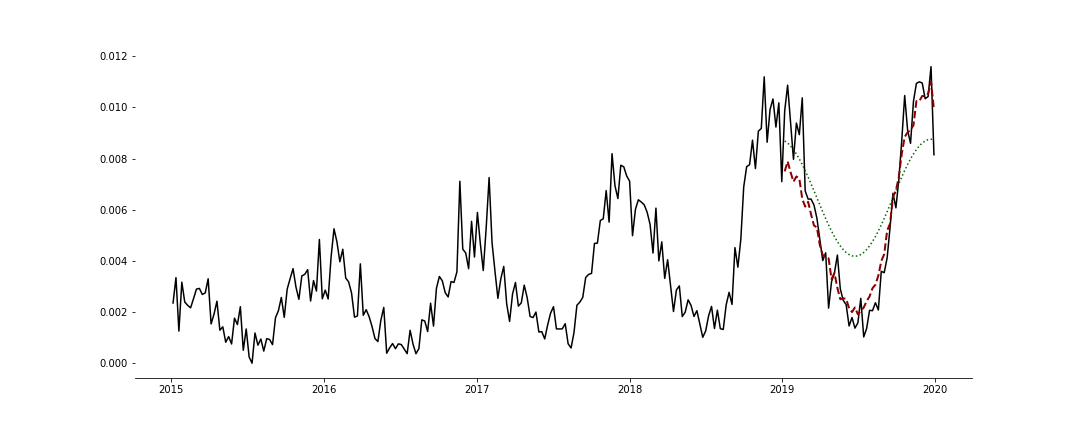
\includegraphics[width=1.\linewidth]{figure/us_female_top}
  %\caption{Time series representing a top fashion trend for female in The United States}
  %\label{fig:examples:sub1}
%\end{subfigure}
%\begin{subfigure}{1.\textwidth}
 % \centering
  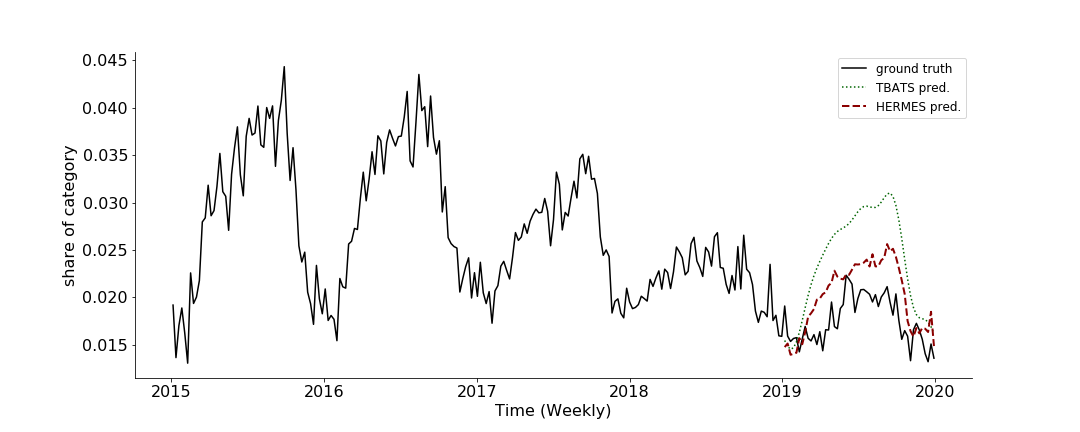
\includegraphics[width=1.\linewidth]{figure/cn_female_texture_horizontalstripe}
  %\caption{Time series representing the horizontal stipes texture fashion trend for female in China}
  %\label{fig:examples:sub2}
%\end{subfigure}
\caption{\textit{hermes-tbats} forecast examples. In green the prediction of the per-time-series predictors \textit{tbats}. In red the final forecast of our HERMES hybrid model \textit{hermes-tbats}. (Top) Time series representing a top fashion trend for female in The United States. (Bottom) Time series representing the horizontal stipes texture fashion trend for female in China.}
\label{fig:examples}
\end{figure*}

\textbf{10000 Heuritech Fashion time series classification task. } The impact of the weak signals are revealed with our classification results. Classification results between the \textit{tbats} model and the hybrid method \textit{hermes-tbats} are given in Table~\ref{tab:tbatsclass}, we note an impresive decrease of impactful errors: forecast an increase instead of a decrease and vice versa. the \textit{hermes-tbats} model divides by 3 the error rate in comparison to \textit{tbats} with only a slightly decrease of the number of correct increase/decrease predictions. However, with our weak signals, we see that \textit{hermes-tbats-ws} is able to catch twice as much as its relative model without weak signal while keeping a relatively low number of impactful errors.

\begin{table}
  \caption{\textit{tbats}, \textit{hermes-tbats} and \textit{hermes-tbats-ws} models confusion matrix }
  %\vspace{0.2cm}
  %\textit{tbats} model confusion matrix \\
  %\par \textit{tbats} model confusion matrix
  %\vspace{0.2cm}
\centering
  \begin{tabular}{l||llll}
  	&& \multicolumn{3}{c}{\textbf{\textit{tbats}}}\\
    && pred-dec  & pred-flat & pred-inc  \\
    \hline
    \hline
    \rule{0pt}{2ex} \\
	true-dec && 902 & 2113 & 327 \\
    true-flat && 351 & 2920 & 300 \\
    true-inc && 300 & 2078 & 709 
  \end{tabular}

\vspace{.2cm}

  \begin{tabular}{l||llll}
  	&& \multicolumn{3}{c}{\textbf{\textit{hermes-tbats}}}\\
    && pred-dec  & pred-flat & pred-inc  \\
    \hline
    \hline
    \rule{0pt}{2ex} \\
	true-dec && 1261 & 1960 & 121 \\
    true-flat && 549 & 2823 & 199 \\
    true-inc && 214 & 2004 & 869 
  \end{tabular}

\vspace{.2cm}

  \begin{tabular}{l||llll}
    && \multicolumn{3}{c}{\textbf{\textit{hermes-tbats-ws}}}\\
    && pred-dec  & pred-flat & pred-inc  \\
    \hline
    \hline
    \rule{0pt}{2ex} \\
	true-dec && 1956 & 1245 & 141 \\
    true-flat && 1257 & 2087 & 227 \\
    true-inc && 358 & 1620 & 1109 
  \end{tabular}
\label{tab:tbatsclass}
\end{table}

\textbf{Size of the dataset. } In addition to the results on the fashion dataset gathering 10000 time series, the behaviour of the HERMES model is analyzed when it is trained on smaller datasets. 2 experiments was done, HERMES models was trained on a reduced dataset of 1000 time series and on a reduced dataset of 100 time series. Results are given in Table~\ref{tab:1000metricresults}.

With these investigations, two important remarks can be done. First, the hybrid framework \textit{hermes-tbats} achieves the first position in term of global accuracy on both datasets. Due to the strengh of its per-time-series predictor TBATS, the hybrid model succeds at correcting some of TBATS weaknesses and logically reach a striking final accuracy. Secondly, we can note that the accuracy of the full neural network \textit{lstm} decreases when the dataset size decreases. On the small dataset of 100 time series, a local statistical model like \textit{tbats} or \textit{stlm} largely outperforms its accuracy level. Learn how to compute a full prediction from scratch is a complex task and high-dimensional recurrent neural networks require  large amount of data. Nevertheless, with the HERMES framework, the RNN task is largely simplified. Our achitectures logicaly needs less data to be trained and to perform well.


\begin{table}
  \caption{Results summary on the 1000ts Fashion dataset and 100ts Fashion Dataset. For each metric, the average on all our time series is computed. For the two approaches using neural network, 10 models with different seeds are trained. the mean and the standard deviation of the 10 results are displayed.}
  \centering
% \resizebox{0.85\textwidth}{!}{ 
  \begin{tabular}{l||llll}
    \multicolumn{4}{c}{1000 ts Fashion dataset}\vspace{0.5cm} \\
    &&\multicolumn{2}{c}{\textbf{MASE}} \\
    &&  \textit{mean}  & \textit{std}  \\
%    \hline
	 \hline
	 &&& \\
     \textit{snaive} && 0.871 & - \\
     \textit{thetam}  && 0.849 & - \\
     \textit{arima} && 0.821 & - \\
     \textit{ets} && 0.801 & - \\
     \textit{stlm} && 0.765 & - \\
     \textit{lstm-nows} && 0.740 & 0.007 \\
     \textit{tbats} && 0.734 & - \\
     \textbf{\textit{hermes-tbats}} && \textbf{0.719} & 0.002 \\
  \end{tabular}

\vspace{.2cm}

  \begin{tabular}{l||llll}
   \multicolumn{4}{c}{100 ts Fashion dataset}\vspace{0.5cm} \\
   &&\multicolumn{2}{c}{\textbf{MASE}} \\
    &&  \textit{mean}  & \textit{std}  \\
%    \hline
	\hline
	 &&& \\
     \textit{snaive} && 0.876 & - \\
     \textit{thetam}  && 0.823 & - \\
     \textit{arima} && 0.814 & - \\
     \textit{ets} && 0.785 & - \\
     \textit{lstm-nows} && 0.767 & 0.045 \\
     \textit{stlm} && 0.742 & - \\
     \textit{tbats} && 0.745 & - \\
     \textbf{\textit{hermes-tbats}} && \textbf{0.739} & 0.003 \\
  \end{tabular}
%  }
\label{tab:1000metricresults}
\end{table}


\subsection{Result for M4 weekly dataset}

In addition to the previous results, a HERMES application is also done on the M4 weekly dataset. The M4 dataset gathers 359 weekly time series and shows 3 main differences compare to the fashion dataset. Firstly, sequences have not the same lenght with sequence lenghts lying between 93 and 2610 time steps. Secondly, as some of the sequences represent financial signals or some others are demographic sequences, the  359 time series show huge contrasting behaviours. Thirldy, compare to the fashion application, the horizon for the M4 competition is set to 13 for the weekly dataset. 

\textbf{Training}

\textcolor{blue}{reformuler}
The sequence are firstly resized in order to egalize their lenghts. For the shorter ones: the eval and the test set is removed (the last 26 steps). Then the remaining number of entire year is duplicated in order to egalize all the sequence at the longest one : 2610 time steps. As per time series parametric model training time depends on the sequence lenght, all time series are then croped. At the end, with the addition of the previously removed eval and test set, 300 time steps are kept for each sequence. 

For this training, The horizon $h$ is set to 13 due to the M4 weekly test set size and the window size $w$ is fixed at 104. For the RNN part, the same architecture than describe in Figure~ \ref{fig:rnn_architecture} is used. The Adam optimizer is used with a learning rate fixed at 0.005 and a batch size set at 8. As the loss function, the same loss than the fashion application is used. As the M4 weekly dataset is small, a rolling window is used on the train set in order to increase the train number of example and improve the training. 5 windows are computed for each sequence for the RNN train set. An overview of our train, eval, test set split and the resizing of the shorter sequences is given in Figure~\ref{}.
The previous parameters: window size, learning rate, batch size and the number of train window per time series are set using a grid search.

\begin{figure*}
  \centering
    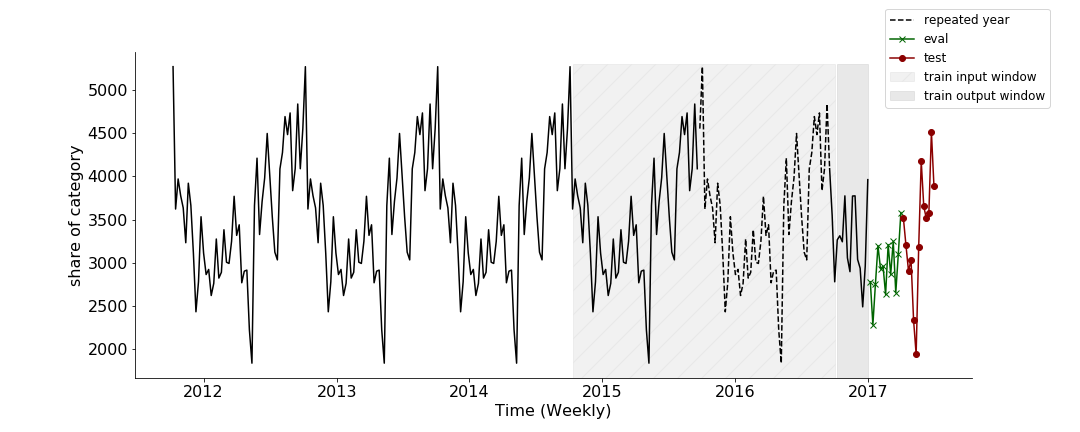
\includegraphics[width=1.\linewidth]{figure/M4_dataset}
  \caption{One of the shortest sequences of the M4 weekly dataset (93 time steps). In order to fit its predictor, the last complete year is duplicated in order to reach a total lenght of 300 time steps.}
\label{fig:m4dataset}
\end{figure*}

\textbf{Benchmarks}

The M4 competion provides a rich collection of benchmarks gatering statistical models and neural network approaches. The same candidates are used in this part as baseline. In addition, the hybrid model named \textit{Uber} of S.Smyl is added to provide an interesting comparison against the HERMES approach. For a complete description and references of the benchmarck models, see \cite{makridakis2020m4}. As a HERMES candidate, a version using TBATS is proposed and called \textit{hermes-tbats}. Following the M4 competition methodology, models are evaluated according to the MASE, the SMAPE and the OWA measure. A complete definition of these metrics is also proposed in \cite{makridakis2020m4}.

\textbf{Results and discussion}

The final results for the M4 weekly dataset are displayed in Table~\ref{tab:m4metricresults}. Considering the HERMES approach, \textit{hermes-tbats} outperforms all the benchmarcks. This results is partially induced by the use of TBATS per-time-series predictors which achieves striking results on the test set. Regarding the hybrid model proposed by S.Smyl, its accuracy remains low in comparison to \textit{tbats} and  \textit{hermes-tbats}. With this second application, two important conclusions can be done. Firstly, the striking results of \textit{hermes-tbats} confirm that the HERMES framework is a general framework, well suited for a large collection of forecasting tasks. Secondly, the accuracy gap between the 2 hybrid candidates validate the HERMES approach and illustrates the importance of a global framework able to leverage any kind of per-time-series predictors.

\begin{table*}
  \caption{Results summary on the m4 weekly dataset. For each metric, the average on all our time series is computed. For approaches using neural network, 10 models are trained with different seeds. The mean and the standard deviation of the 10 results are displayed.}
  \centering
 % \resizebox{0.85\textwidth}{!}{%
  \begin{tabular}{l||lllll|lllll|lllll}
   &&\multicolumn{3}{c}{\textbf{SMAPE}} &&& \multicolumn{3}{c}{\textbf{MASE}} &&& \multicolumn{3}{c}{\textbf{OWA}}&\\
    &&  \textit{mean}  && \textit{std} &&&  \textit{mean}  && \textit{std}&&&  \textit{mean}  && \textit{std}& \\
%    \hline
	 \hline
	 &&&&&&&&&&\\
     \textit{MLP} && 21.349 && - &&& 13.568 && - &&& 3.608 && - &\\
     \textit{RNN} && 15.220 && - &&& 5.132 && - &&& 1.755 && - &\\
     \textit{snaive} && 9.161 && - &&& 2.777 && - &&& 1.000 && - &\\
     \textit{SES} && 9.012 && - &&& 2.685 && - &&& 0.975 && - &\\
     \textit{Theta} && 9.093 && - &&& 2.637 && - &&& 0.971 && - &\\
     \textit{Holt} && 9.708 && - &&& 2.420 && - &&& 0.966 && - &\\
     \textit{Com} && 8.944 && - &&& 2.432 && - &&& 0.926 && - &\\
     \textit{Damped} && 8.866 && - &&& 2.404 && - &&& 0.917 && - &\\
     \textit{Uber} && 7.817 && - &&& 2.356 && - &&& 0.851 && - &\\
     \textit{tbats} && 8.111 && - &&& 2.214 && - &&& 0.8 && - &\\
     \textit{\textbf{hermer-tbats}} && \textbf{7.597} && 0.113 &&& \textbf{2.205} && 0.042 &&& \textbf{0.812} && 0.011 &\\
    %\hline
  \end{tabular}
%  }
\label{tab:m4metricresults}
\end{table*}


\section{Conclusion}
\label{sec:conclusion}
The motivation of this paper was to present HERMES, a new hybird model for time series forecasting. This new framework is a really promising approach. By mixing the performance of local parametric models and a global neural network. The \textit{hermes-tbats} version clearly outperform traditional statistical methods and full neural network models. Furthermore, this new model is totally suited for dealing with external signals. With a fine pre-processing and a well-designed architecture, our hybrid framework succeed at leveraging our complex extra data and reach impressive accuracy level in term of classification. In addition to this article, a fashion dataset gathering a sample of $\numberts$ time series and a collection of weak signals is provided. We believe that this dataset hide really fine dynamics and interactions where complex models would express their potential. By making it publicly available, we hope that it will enhance the set of datasets for time series forecasting and pave the way for further explorations.
As a possible future work, a different inclusion of the weak signals can be design in the HERMES architecture. Focusing on the example with huge change of behaviors, a fine analysis of the predictive power of the collection of weak signals can be done. In the same way, an interesting improvment of the hybrid framework can be to introduce not a single but several neural networks trained at correcting different kinds of weaknesses and activate or not by a latent space. This latent space can be drive by the historical data or even more by the weak signals.


\appendices

%\renewcommand{\thetable}{A\arabic{table}}
%\renewcommand{\thefigure}{A\arabic{figure}}
%\setcounter{table}{0}
%\setcounter{figure}{0}


\section{M4 weekly dataset and results}


\section{Training parameters and loss}


\subsection{Loss grid search on the Fashion Dataset}

Using deep learning models in time series forecasting is a appealing way to achieve higher levels of accuracy. However, it induces two main issues. First, have a large enough dataset to train the model as illustrated in Section~\ref{sec:exp}. Second, find a correct loss to train the model. For the second point, the main difficulty is that a dataset can gather contrasting time series in terms of scale. These differences can impact the loss behaviour and finally the training. For the HERMES architecture, some loss candidates were defined for the training : the Mean Absolute Error (MAE), the Mean Square Error (MSE),  the Scaled Mean Absolute Error (SMAE) and the Scaled Mean Square Error (SMSE).
The loss functions are defined as follows :


$$
MAE = \frac{1}{\lag}\sum_{i=1}^{\lag}|\ts^n_{T+i} - \tspred^n_{T+i|T}|\,,\quad  MSE = \frac{1}{\lag}\sum_{i=1}^{\lag}|\ts^n_{T+i} - \tspred^n_{T+i|T}|
$$
$$
SMAE = \frac{1}{\meants^n_T}\sum_{i=1}^{\lag}|\ts^n_{T+i} - \tspred^n_{T+i|T}|\,,\quad  SMSE = \frac{1}{\meants^n_T}\sum_{i=1}^{\lag}|\ts^n_{T+i} - \tspred^n_{T+i|T}|
$$

For each loss, 10 \textit{hermese-tbats-ws} models have been trained with different seeds and the final mean and standard deviation are given in Figure~\ref{}. The final Scaled Mean Absolute Error reach the lower MASE and was selected to train all the HERMES model in this paper.

\begin{figure}
  \centering
    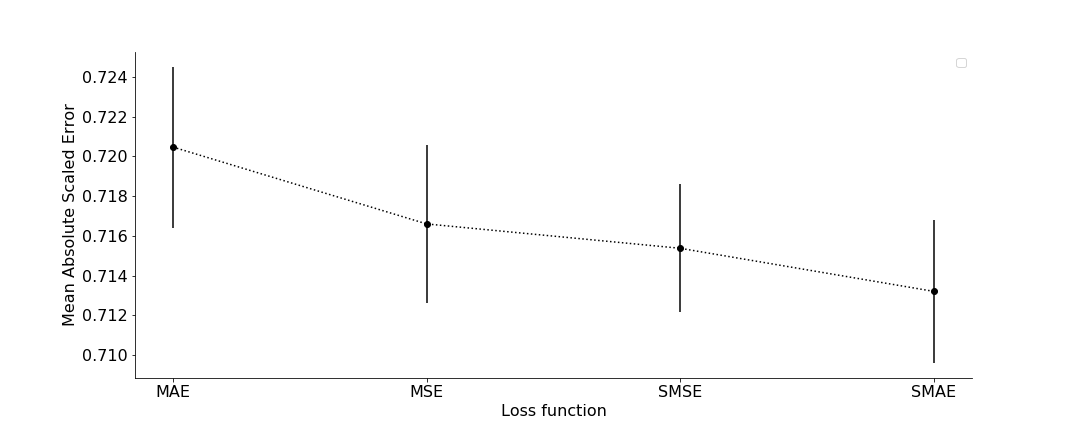
\includegraphics[width=1.\linewidth]{figure/loss_function}
  \caption{MASE accuray for the \textit{hermes-tbats-ws} model depending of the loss used during the RNN training. For each loss, 10 models with different seed have been trained. The mean and the standard deviation are represented with a point and a vertical line.}
\label{fig:loss_function}
\end{figure}



\subsection{Parameters grid search on the M4 weekly Dataset}

The HERMES framework get several parameters to set correctly in order to reach acceptable level of accuracy. For instance, a overview of the learning rate, batch size and number of window per time series grid search for the M4 weekly dataset is shown in this part. For each parameters, a collection of 10 \textit{hermes-tbats} models have been trained with a range of values and the final OWA was calculated. As in the Figure~\ref{fig:loss_function}, the mean and the standard deviation of each groups of 10 trainings is displayed in Figure~\ref{}. For the final \textit{hermes-tbats} model of the M4 weekly dataset, the grid search fixed the following setup : 3 windows per time series, the batch size set to 8 and the optimizer's learning rate equal to 0.005.

 
\begin{figure}
\centering
%\begin{subfigure}{1.\textwidth}
 % \centering
  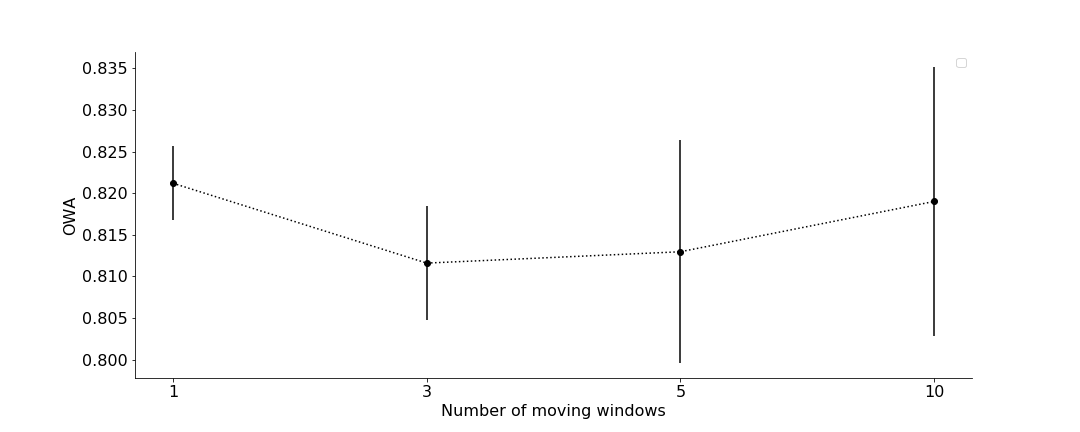
\includegraphics[width=1.\linewidth]{figure/m4_nb_of_window}
  %\caption{result of the HERMES model on the M4 dataset model depending of the number of windows provided per time series to the RNN corrector}
 % \label{fig:m4parameter:sub1}
%\end{subfigure}
%\begin{subfigure}{1.\textwidth}
 % \centering
  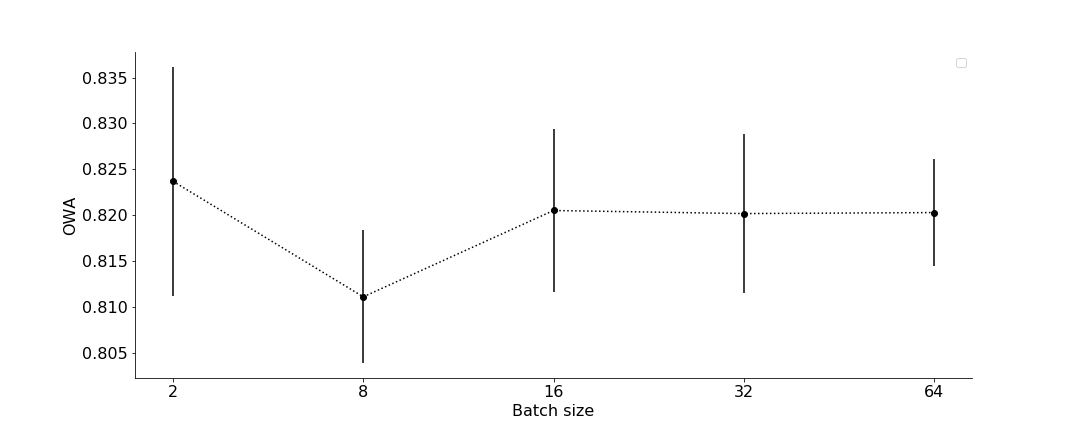
\includegraphics[width=1.\linewidth]{figure/m4_batch_size}
  %\caption{result of the HERMES model on the M4 dataset model depending of the size of the batch size}
  %\label{fig:m4parameter:sub2}
%\end{subfigure}
%\begin{subfigure}{1.\textwidth}
  %\centering
  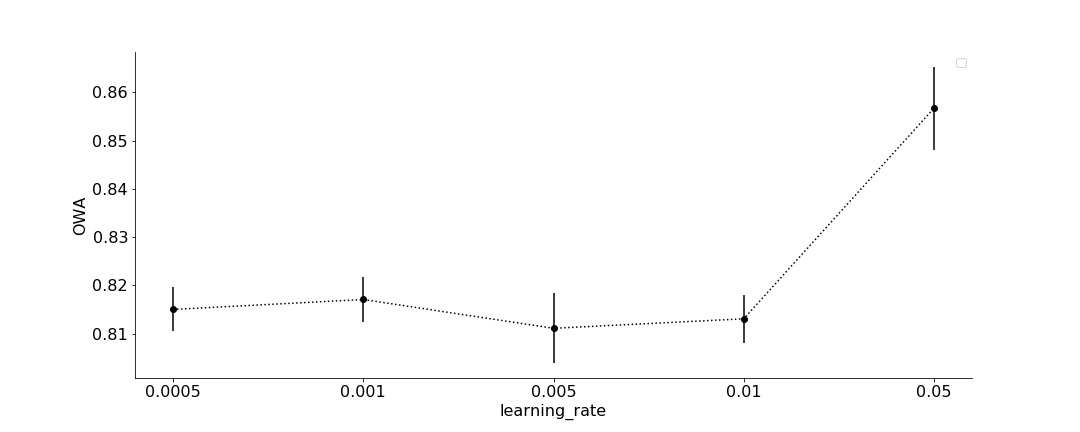
\includegraphics[width=1.\linewidth]{figure/m4_learning_rate}
  %\caption{result of the HERMES model on the M4 dataset model depending of learning rate of the optimizer}
  %\label{fig:m4parameter:sub3}
%\end{subfigure}
\caption{Example of difference between the raw sequence and the normalized one. In this example, we normalize by the deseasonalized global top fashion trend for female in China. (Top) result of the HERMES model on the M4 dataset model depending of the number of windows provided per time series to the RNN corrector. (Middle) Result of the HERMES model on the M4 dataset model depending of the size of the batch size. (Bottom) Result of the HERMES model on the M4 dataset model depending of learning rate of the optimizer.}
\label{fig:m4parameter}
\end{figure}


% use section* for acknowledgment
%\section*{Acknowledgment}
%
%
%The authors would like to thank...


% Can use something like this to put references on a page
% by themselves when using endfloat and the captionsoff option.
% \ifCLASSOPTIONcaptionsoff
%   \newpage
% \fi
\newpage


% trigger a \newpage just before the given reference
% number - used to balance the columns on the last page
% adjust value as needed - may need to be readjusted if
% the document is modified later
%\IEEEtriggeratref{8}
% The "triggered" command can be changed if desired:
%\IEEEtriggercmd{\enlargethispage{-5in}}

% references section

% can use a bibliography generated by BibTeX as a .bbl file
% BibTeX documentation can be easily obtained at:
% http://mirror.ctan.org/biblio/bibtex/contrib/doc/
% The IEEEtran BibTeX style support page is at:
% http://www.michaelshell.org/tex/ieeetran/bibtex/
\bibliographystyle{IEEEtran}
% argument is your BibTeX string definitions and bibliography database(s)
\bibliography{hermes_paper}
%
% <OR> manually copy in the resultant .bbl file
% set second argument of \begin to the number of references
% (used to reserve space for the reference number labels box)
%\begin{thebibliography}{1}
%
%\bibitem{IEEEhowto:kopka}
%H.~Kopka and P.~W. Daly, \emph{A Guide to \LaTeX}, 3rd~ed.\hskip 1em plus
%  0.5em minus 0.4em\relax Harlow, England: Addison-Wesley, 1999.
%
%\end{thebibliography}

% biography section
%
% If you have an EPS/PDF photo (graphicx package needed) extra braces are
% needed around the contents of the optional argument to biography to prevent
% the LaTeX parser from getting confused when it sees the complicated
% \includegraphics command within an optional argument. (You could create
% your own custom macro containing the \includegraphics command to make things
% simpler here.)
%\begin{IEEEbiography}[{\includegraphics[width=1in,height=1.25in,clip,keepaspectratio]{mshell}}]{Michael Shell}
% or if you just want to reserve a space for a photo:

%\begin{IEEEbiography}{Michael Shell}
%Biography text here.
%\end{IEEEbiography}

% if you will not have a photo at all:
%\begin{IEEEbiographynophoto}{John Doe}
%Biography text here.
%\end{IEEEbiographynophoto}

% insert where needed to balance the two columns on the last page with
% biographies
%\newpage

%\begin{IEEEbiographynophoto}{Jane Doe}
%Biography text here.
%\end{IEEEbiographynophoto}

% You can push biographies down or up by placing
% a \vfill before or after them. The appropriate
% use of \vfill depends on what kind of text is
% on the last page and whether or not the columns
% are being equalized.

%\vfill

% Can be used to pull up biographies so that the bottom of the last one
% is flush with the other column.
%\enlargethispage{-5in}



% that's all folks
\end{document}
